%%%%%%%%%%%%%%%%%%%%%%%%%%%%%%%%%%%%%%%%%%%%%%%%%%%%%%%%%%%%%%%%%%%%%%%%
%  ICLR 2027 SUBMISSION
%  Flow-Aligned Distillation: Preserving Layer-Wise Residual
%  Trajectories in Compressed Language Models
%
%  BUILD:  pdflatex fad ; bibtex fad ; pdflatex fad ; pdflatex fad
%  STATUS: public artifact source containing the main paper and appendix.
%
%  ---------------------------------------------------------------------
%  ICLR 2027 RULES THIS FILE IS BUILT AGAINST
%  (source: https://iclr.cc/Conferences/2027/AuthorGuidelines)
%  ---------------------------------------------------------------------
%   * Abstract deadline  Sept 11 2026 AOE; full paper Sept 16 2026 AOE;
%     decisions Dec 9 2026.  No authors may be ADDED after Sept 11.
%   * Main text <= 9 pages at submission (10 for rebuttal/camera-ready).
%     Strictly enforced; over-length papers are DESK-REJECTED.
%   * References do not count and are unlimited.
%   * Double blind.  Author identity revealed in the main text OR in the
%     supplementary material => desk rejection.  Self-citation must be in
%     the third person.
%   * AI Use Statement: REQUIRED, does not count toward the page limit.
%   * Reproducibility Statement: recommended, placed at the end of the
%     main text BEFORE the references, does not count toward the limit.
%   * Ethics Statement: optional, same placement, <= 1 page, does not
%     count toward the limit.
%   * Official template: https://github.com/ICLR/Master-Template/raw/master/iclr2027.zip
%   * Dual submission: parallel submission of substantially similar work
%     is prohibited for the whole review period.  Do NOT have the ICASSP
%     compression manuscript under review at the same time as this paper.
%
%  ---------------------------------------------------------------------
%  WHAT CHANGED IN THIS REVISION (per ICLR2027_full_review_and_rewrite.md)
%  ---------------------------------------------------------------------
%  1. Single story.  The paper now answers exactly one question: given a
%     structurally compressed transformer, which layer-wise signal should
%     be distilled?  Shared-FFN compression is a *fixed testbed*, and the
%     adaptive-exit runtime mechanism has been moved out of the abstract,
%     the contributions, the main text and the conclusion into
%     the supplementary material (Sec. S7).
%  2. Terminology unified.  Everywhere we now say "discrete layer-wise
%     residual trajectory", "local transport increment / velocity" and
%     "trajectory drift".  The terms "one-step", "rectified target",
%     "information energy", "surprisal" and "moments" have been removed.
%  3. PCA is no longer self-contradictory.  Sec.~\ref{sec:geometry} now
%     separates (a) subspace *selection* -- which directions are modeled --
%     from (b) within-subspace *standardization* -- how errors are compared
%     among retained directions.
%  4. The derivation in the main text is the short chain
%     Barber--Agakov -> maximum-entropy Gaussian -> Mahalanobis loss.
%     The Lagrangian, strict concavity and uniqueness argument now live in
%     the supplementary material (Sec. S3).
%  5. Two assignment maps are now typographically distinct:
%     c(\ell) = coordinate group (PCA basis),
%     g(\ell) = parameter-sharing group (shared FFN bank).
%  6. All "in the supplement" pointers now resolve to real, written
%     sections of ICLR2027_supplementary.tex.
%
%  ---------------------------------------------------------------------
%  BEFORE SUBMISSION -- MANDATORY AUTHOR ACTIONS
%  ---------------------------------------------------------------------
%  [ ] Replace iclr2027_conference.sty with the OFFICIAL ICLR 2027 kit
%      (https://github.com/ICLR/Master-Template/raw/master/iclr2027.zip)
%      and recompile BOTH this file and the supplementary file; re-check
%      the 9-page main-text limit.  Do not adjust margins, font size or
%      line spacing to fit.
%  [ ] Add the mandatory AI Use Statement.  A ready-to-paste block is kept
%      commented out just before the Reproducibility Statement below.
%      (Deliberately left commented out at the author's request.)
%  [ ] Confirm the exact Qwen release name / HF revision (supplementary S1).
%  [ ] Fill the cells marked \tba in Tables~\ref{tab:objective}
%      and~\ref{tab:drift} and produce Figure~\ref{fig:drift}.
%  [ ] Check the supplementary PDF for author-identifying metadata too:
%      anonymity is enforced on the supplement as well.
%
%  ---------------------------------------------------------------------
%  RESULTS AUDIT -- NUMBERS THAT DISAGREE ACROSS PAPER / THESIS / SLIDES
%  ---------------------------------------------------------------------
%  The numbers below are the ones used in this file.  Each is flagged
%  %% AUDIT at its point of use.  Resolve every conflict against a single
%  results manifest before the submission deadline.
%    (a) Metric ablation macro gain:  +8.14 pp (0.7752 -> 0.8566) here,
%        but +4.49 pp (0.7752 -> 0.8202) in the thesis, same 19/28 setting.
%    (b) Adaptive-exit speedup: 1.463x in the supplementary material,
%        1.388x in the thesis.
%    (c) Adaptive-exit average executed depth: 16.39 here, 17.95 in the
%        thesis' detailed 20% study.
%    (d) "25% budget": state once whether this is the removed fraction,
%        the retained fraction, or a total-model reduction target.
%%%%%%%%%%%%%%%%%%%%%%%%%%%%%%%%%%%%%%%%%%%%%%%%%%%%%%%%%%%%%%%%%%%%%%%%
\documentclass{article}

\usepackage{iclr2027_conference,times}
% \iclrfinalcopy   % <-- uncomment for camera-ready only

% \usepackage[hyphens]{url}
\usepackage{hyperref}
\usepackage{url}
\usepackage{graphicx}
\usepackage{natbib}
\usepackage{amsmath,amssymb,amsfonts,amsthm}
\usepackage{mathtools}
\usepackage{booktabs}
\usepackage{tabularx}
\usepackage{float}
\usepackage{caption}
\usepackage{subcaption}
\usepackage{microtype}
\usepackage{placeins}
% \urlstyle{rm}
\captionsetup{font=small}
\usepackage{placeins}

% ---------------------------- macros ----------------------------------
\newcommand{\E}{\mathbb{E}}
\newcommand{\R}{\mathbb{R}}
\newcommand{\calH}{\mathcal{H}}
\newcommand{\calL}{\mathcal{L}}
\newcommand{\calS}{\mathcal{S}}
\newcommand{\calG}{\mathcal{G}}
\newcommand{\calN}{\mathcal{N}}
\newcommand{\calQ}{\mathcal{Q}}
\newcommand{\FAD}{\mathrm{FAD}}
\newcommand{\CE}{\mathrm{CE}}
\newcommand{\KL}{\mathrm{KL}}
\newcommand{\NLL}{\mathrm{NLL}}
\newcommand{\Attn}{\mathrm{Attn}}
\newcommand{\Norm}{\mathrm{Norm}}
\newcommand{\FFN}{\mathrm{FFN}}
\newcommand{\Var}{\mathrm{Var}}
\newcommand{\Cov}{\mathrm{Cov}}
\newcommand{\Diag}{\operatorname{Diag}}
\newcommand{\bB}{\boldsymbol{B}}
\newcommand{\bs}{\boldsymbol{s}}
\newcommand{\bz}{\boldsymbol{z}}
\newcommand{\bv}{\boldsymbol{v}}
\newcommand{\by}{\boldsymbol{y}}
\newcommand{\bmu}{\boldsymbol{\mu}}
\newcommand{\bsigma}{\boldsymbol{\sigma}}
\newcommand{\bveps}{\boldsymbol{\varepsilon}}
\newcommand{\bSigma}{\varSigma}
\newcommand{\bI}{I}
% Placeholder for a cell that must be filled from a dedicated experiment.
\newcommand{\tba}{\textit{--}}
\theoremstyle{plain}
\newtheorem{theorem}{Theorem}
\newtheorem{proposition}[theorem]{Proposition}
\theoremstyle{definition}
\newtheorem{definition}{Definition}
\theoremstyle{remark}
\newtheorem{remark}{Remark}
\newtheorem{assumption}[theorem]{Assumption}

\graphicspath{{.}{./Figure/}{./figures/}}
\newcommand{\paperfig}[2]{%
  \IfFileExists{#1}{\includegraphics[width=#2]{#1}}{%
    \fbox{\parbox[c][2.4cm][c]{#2}{\centering\ttfamily\footnotesize
      [figure placeholder]\\ \detokenize{#1}}}}}
% ======================================================================

\title{Flow-Aligned Distillation: Preserving Layer-Wise Residual Trajectories in Compressed Language Models}

\author{Anonymous authors\\Paper under double-blind review}

\begin{document}
\maketitle

% ======================================================================
\begin{abstract}
% ======================================================================
A large portion of the parameters in a transformer are allocated by feed-forward network (FFN) layers. Compressing a transformer via FFN accordingly alters the residual update at each layer, and the resulting local mismatches can propagate through depth. The evolution of the residual stream across the transformer layers is viewed as a \emph{trajectory in} layers. Within each block, the post-attention state is linearly interpolated with the next-layer hidden state. The derivative along this interpolation is constant and equals the FFN residual update, which is seen as the local velocity of the transition. Flow-aligned distillation (FAD) is proposed by aligning these local velocities between the teacher and the student. FAD projects these velocities into a low-rank coordinate system estimated from frozen teacher velocities, where the projected deviations are using the inverse square root of a layer-wise diagonal covariance estimated from the teacher. Starting from a variational lower bound on mutual information, this paper presents a maximum-entropy conditional model whose conditional mean is the projected student velocity and whose covariance is formed by the projected teacher velocities. Solving this problem corresponds to maximizing a Gaussian conditional or minimizing a Mahalanobis alignment loss. The coordinate system is therefore estimated from the teacher and is derived through the relative inverse-variance weighting across projected directions. To investigate the effect of the distillation objective, we compare competing losses in identical architectures with shared FFN weights, training data, and optimization settings. Using Llama-3.2-3B and Llama-3.1-8B, FAD outperforms distillation at the logit-level and hidden-state matching. It also improves over matched-compression baselines while reducing model parameters by $20.93\%$ at the primary operating point. These results support aligning FFN-induced local transitions along the layer-wise trajectory as an effective principle for capability recovery in structurally compressed language models.
\end{abstract}

\begin{figure}[t] \centering
  \paperfig{Figure/fad.pdf}{0.96\linewidth}
  \caption{\label{fig:pipeline}Overview of flow-aligned distillation (FAD) with three stages. The frozen teacher (top) and the compressed student (bottom) process the same input, and at the {last prediction token} $T$, each block $\ell$ exposes its FFN residual update as a one-step transport velocity, $v_T^{(\ell)}=\Delta h_T^{(\ell)}$ and $v_S^{(\ell)}=\Delta h_S^{(\ell)}$. {(a)}~Attention is frozen in both models; teacher keeps its $L$ independent FFNs, whereas student replaces them with \emph{shared} weights together with a trainable per-layer low-rank adapter by Eq.\eqref{eq:student-ffn}, and layers with similar FFN inputs are tied to a single core (the colored ``Shared FFN Parameter'' blocks: red, yellow and green indicate three parts of sharing). {(b)}~A shared low-rank teacher basis (``project~$\bB$'') maps both velocities to their subspace codes $\{\bz_T^{(\ell)}, \bz_S^{(\ell)}\}$ by Eq.\eqref{eq:proj}. {(c)}~Flow-aligned distillation pulls the student transport (blue) onto the teacher transport (red) layer by layer; the training signal is the teacher-induced information-theoretic objective, which is arranged as FAD loss by Eq.\eqref{eq:fad}.}
\end{figure}
%{Flow-aligned distillation preserves a discrete layer-wise residual trajectory.} At each supervised layer $\ell$, the FFN residual ($\triangle h^{(\ell)}$) update is treated as the local increment of the model's residual trajectory. Teacher (red) and student (blue) increments are projected into a teacher-derived subspace and compared after layer-wise variance matching. The shared-FFN student is the controlled structural compression setting used to evaluate this distillation signal.

% ======================================================================
\section{Introduction}
\label{sec:intro}
% ======================================================================

Structural compression reduces the model storage, but also perturbs the computation performed at each layer. In a residual transformer, such perturbations can propagate through depth because each block consumes the state produced by the preceding blocks. In previous methods \citep{romero2015fitnets,jiao2020tinybert,wang2020minilm,sanh2019distilbert,
gu2024minillm,agarwal2024gkd}, the output-logit distillation might constrain the final prediction, whereas the hidden-state matching might constrain the representations reached in the selected layers. Neither of them directly supervised the feed-forward network (FFN) update that transformed the post-attention state into the next-layer hidden state. We therefore argue whether the local quantity in a compressed student should be reproduced to follow the teacher's computation across layers.

Consequently, we view the evolution of the residual stream across transformer layers as a trajectory in the layer-wise direction. Within each block, the residual FFN update connects the post-attention state to the next-layer hidden state. The derivative of the corresponding straight-line interpolation is constant and equals this update, giving it a local velocity interpretation. This motivates aligning teacher and student FFN velocities rather than matching only the final outputs or the hidden states. This paper presents flow-aligned distillation (FAD), which compares these velocities in a geometry estimated from the frozen teacher. FAD projects teacher and student velocities into teacher-derived low-rank coordinates and accounts for their layer-wise directional scales. A variational mutual-information bound \citep{barber2003im,poole2019variational}, together with a maximum-entropy conditional model
\citep{jaynes1957information}, yields a Gaussian conditional which results in a Mahalanobis alignment objective. To evaluate the distillation signal, all compared methods use the same shared-weight student architecture, frozen teacher, training data, and
optimization protocol. There are three-fold findings which are presented to
\begin{itemize}
\item[$-$] interpret the transformer's FFN residual updates as the one-step local transport velocities and formulate the shared-FFN compression as the preservation of teacher transport information under a parameter budget,
\item[$-$] combine the teacher-derived low-rank coordinates with the layer-wise directional normalization to obtain the FAD objective,
\item[$-$] match or even outperform the performance of teacher model using the compressed FAD models where FFN parameters are compressed, and validates over different information-theoretic transport targets, teacher-derived transport coordinates, and teacher-induced scale matrix.
\end{itemize}

% ======================================================================
\section{Related Work}
\label{sec:related}
% ======================================================================

\paragraph{Structural compression and parameter sharing.}
Quantization \citep{jacob2018quantization,frantar2023gptq,lin2023awq}, pruning \citep{han2015deepcompression,frantar2023sparsegpt,sun2024wanda,ma2023llmpruner}, layer removal \citep{men2024shortgpt,chen2025streamlining,flatllm,flap} and weight tying \citep{lan2020albert,dehghani2019universal, shareyourattention,flexigpt} reduce the model cost through different structural constraints. Their optimization criteria are developed primarily through parameter or activation reconstruction or saliency, or end-to-end task loss. These criteria can preserve the overall quality of the model, but none of them explicitly supervises the residual update produced by each compressed layer. The proposed FAD aims to provide a layer-wise recovery signal for a fixed compressed architecture, which consolidates {FFN} operators based on shared structural banks, leaving attention and logical depth unchanged.

\paragraph{Intermediate knowledge distillation.}
Knowledge distillation is commonly performed for model compression by matching output distributions, hidden states, attention relations, or student-generated sequences \citep{romero2015fitnets,jiao2020tinybert,wang2020minilm,sanh2019distilbert,
gu2024minillm,agarwal2024gkd}. This study similarly preserves the intermediate variables. Rather than matching a complete hidden state, this paper matches the FFN residual update that mimics the teacher's residual trajectory. It also separates coordinate selection from error scaling: both models are projected into teacher-derived velocity coordinates, and their deviations are standardized by the layer-wise teacher covariance. Where a feature-matching loss using its weights is usually chosen and tuned, here all three choices including variable, coordinate, and scale follow from the same variational objective.

\paragraph{Flow matching and information bottleneck.}
Flow matching is feasible to enable learning by aligning the velocity along a prescribed path \citep{chen2018neuralode,lipman2023flowmatching, liu2023rectified}. This study would like to capture the geometric information from a teacher based on the realized residual increment at each layer in a way that a student is learned for information preservation. In \citep{barber2003im,poole2019variational}, the variational mutual-information bounds were derived to validate the information bottleneck, which is referred to illustrate the proposed FAD for the compression-prediction trade-off between teacher velocities as the source information, student velocities as the target representation, and a finite rank budget forcing the dominant teacher directions to be sufficiently preserved.

% ======================================================================
\section{Flow-Aligned Distillation}
\label{sec:method}
% ======================================================================

This paper deals with model compression by aligning the teacher and student large language models (LLMs) based on their FFN residual updates in a low-rank geometry built by the frozen teacher. We first define the aligned variable, then construct its teacher-derived coordinates and directional scales, and finally derive the alignment objective. The shared-weight student is implemented in the fixed structural-compression setting. However, the derived FAD objective does not depend on a particular parameter-sharing assignment. Throughout, $L$ denotes the number of layers and $D$ the dimension of the features. The subscripts $T$ and $S$ indicate the teacher and the student, respectively. The map $c:[L]\to[Q]$ assigns a layer to a coordinate of $Q$ groups, while $g:[L]\to[K]$ assigns it to the $K$ parameter-sharing groups. Velocities are extracted at the final non-padding input position used to predict the next token.

\subsection{FFN Residual Update as Local Velocity}
\label{sec:trajectory}

For the distillation model $M\in\{T,S\}$ and the input sequence $x$, let $\calH_M(x)=\bigl(h_M^{(1)},\ldots,h_M^{(L+1)}\bigr)$ denote its discrete layer-wise trajectory of hidden states $h_M^{(\ell)}$. The $\ell$-th pre-norm block or layer first produces the post-attention state $u_M^{(\ell)}$ and then updates it as $\Delta h_M^{(\ell)}$ through the FFN
\begin{equation} \begin{aligned}
  u_M^{(\ell)} = h_M^{(\ell)} + \Attn_M^{(\ell)} \bigl(
    \Norm_1(h_M^{(\ell)}) \bigr),~~ \Delta h_M^{(\ell)} =
  \FFN_M^{(\ell)} \bigl( \Norm_2(u_M^{(\ell)}) \bigr),~~
  h_M^{(\ell+1)} = u_M^{(\ell)} + \Delta h_M^{(\ell)}
\end{aligned} \label{eq:block-transition} \end{equation}
where two normalizations are performed on $h_M^{(\ell)}$ and $u_M^{(\ell)}$, respectively. The residual update of FFN $\Delta h_M^{(\ell)}$ is therefore the displacement from the post-attention state $u_M^{(\ell)}$ to the hidden state of the next-layer $h_M^{(\ell+1)}$. In particular, the layer-wise flow transition $\phi_M^{(\ell)}(t)$, where $t\in[0,1]$, is represented by a linear interpolation, where its local velocity $\bv_M^{(\ell)}$ is defined by differentiation as follows
\begin{equation} \begin{aligned}
  \phi_M^{(\ell)}(t) = u_M^{(\ell)} + t\Delta h_M^{(\ell)},\quad \bv_M^{(\ell)} \triangleq \frac{\partial\phi_M^{(\ell)}(t)} {\partial t} = \Delta h_M^{(\ell)}.
\end{aligned} \label{eq:local-velocity} \end{equation}
FAD aligns the velocities $\bv_T^{(\ell)}$ and $\bv_S^{(\ell)}$ at the supervised layers. Their mismatch changes the next-layer hidden state and can therefore propagate to subsequent blocks.

% ----------------------------------------------------------------------
\subsection{Teacher-Induced Coordinate and Scale}
\label{sec:geometry}
% ----------------------------------------------------------------------

Having induced $\bv_M^{(\ell)}$ as the local quantity to be aligned, we next evaluate how teacher-student velocity deviations are measured. An unweighted Euclidean loss in $\R^D$ treats individual full-space directions equally, despite the strongly non-uniform variations of teacher FFN updates. This method runs two operations: selecting a low-rank coordinate system and standardizing deviations within that system.

\paragraph{Teacher-induced coordinate.}
Layers with similar teacher-velocity statistics are assigned to one of the $Q$ coordinate groups through $c:[L]\to[Q]$. For each group $c$, a coordinate based on the rank-$r$ orthonormal PCA basis is constructed through a projection $\bB_c\in\R^{D\times r}$ with teacher mean $\bmu_c\in\R^D$ from frozen teacher velocities $\bv_{T,n}^{(\ell)}$ of the sample $n$. Teacher and student velocities are projected using the same basis and centroid
\begin{equation} \label{eq:proj}
  \bz_{M,n}^{(\ell)} = \bB_{c(\ell)}^{\top} (\bv_{M,n}^{(\ell)} - \bmu_{c(\ell)}
  ) \in\R^r, \qquad M\in\{T,S\}.
\end{equation}
This projection restricts the alignment objective to the leading directions of the teacher-velocity variations. The same centroid is applied to both models, resulting in the projected deviation
\[ \bz_{S,n}^{(\ell)} - \bz_{T,n}^{(\ell)} = \bB_{c(\ell)}^{\top} \bigl(\bv_{S,n}^{(\ell)} - \bv_{T,n}^{(\ell)} \bigr). \]

\paragraph{Layer-wise normalization.}
The projected teacher velocities still have substantially different scales or variances in coordinates and layers. Without normalization, high-variance coordinates would result in the loss and its gradients. We therefore estimate the layer-wise diagonal covariance matrix
\begin{equation}
  (\bsigma_T^{(\ell)})^2 = \Var_n \bigl[\bz_{T,n}^{(\ell)} \bigr], \qquad \bSigma_T^{(\ell)} = \Diag ((\bsigma_T^{(\ell)})^2 ) + \epsilon\bI_r \succ 0
  \label{eq:teacher-covariance}
\end{equation}
where $\bI_r$ is the identity matrix, $\epsilon>0$ prevents division by zero and ensures that $\bSigma_T^{(\ell)}$ is positive definite. In alignment loss, projected deviations are normalized by $(\bSigma_T^{(\ell)})^{-1/2}$, which inducing the precision metric $(\bSigma_T^{(\ell)})^{-1}$. Thus, the PCA basis determines which teacher-velocity directions are modeled, while the layer-wise covariance determines how deviations along those directions are weighted. All teacher-derived statistics are estimated once and kept fixed during student training.

% ----------------------------------------------------------------------
\subsection{From Information Preservation to Flow Alignment}
\label{sec:derivation}
% ----------------------------------------------------------------------

For each supervised layer $\ell\in\calS$ from the teacher, let $p_\ell(\bz_T^{(\ell)},\bz_S^{(\ell)})$ denote the joint distribution of the projected teacher and student velocities induced by the training data. FAD estimates the shared-weight student $\theta_S^\star$ under $\Theta_{\mathrm{shared}}$ that maximizes mutual information (MI) $I(\cdot)$ between projected teacher and student velocities and minimizes Kullback-Leibler (KL) divergence using layer-wise distribution ${p_\ell}(\cdot)$
\begin{equation}
\resizebox{\linewidth}{!}{$\displaystyle \theta_S^\star = \underset{\theta_S\in\Theta_{\mathrm{shared}}} {\operatorname{arg\,max}}
\frac{1}{|\calS|} \sum_{\ell\in\calS} \left[I_{p_\ell} \bigl(\bz_T^{(\ell)}; \bz_S^{(\ell)}
\bigr) - \E_{p_\ell(\bz_S^{(\ell)})} [ \KL( p_\ell (\bz_T^{(\ell)} | \bz_S^{(\ell)} ) \Vert q_{\theta_S}^{\star}
  (\bz_T^{(\ell)} | \bz_S^{(\ell)} ) ] \right]$}
\label{eq:information-objective}
\end{equation}
where the conditional variational model $q_{\theta_S}^{\star}$ is calculated with the highest entropy $H_q(\cdot)$ via
\begin{equation}
q_{\theta_S}^{\star} = \underset{q\in\calQ_{\theta_S}^{(\ell)}} {\operatorname{arg\,max}} ~H_q \bigl(\bz_T^{(\ell)} | \bz_S^{(\ell)} \bigr), \qquad \forall\,\ell\in\calS.
\label{eq:maxent-conditional}
\end{equation}
In Eqs.~\eqref{eq:information-objective} and~\eqref{eq:maxent-conditional}, the student velocities are favored to preserve information about the paired teacher velocities. The KL term measures the gap between the real posterior $p_\ell(\cdot)$ and the variational posterior $q_{\theta_S}(\cdot)$ associated with the current student. The conditional model is specified without introducing an auxiliary inference network. The admissible variational densities satisfy
\begin{equation}
\calQ_{\theta_S}^{(\ell)} = \left\{q: \begin{array}{l}
q\bigl(\bz_T^{(\ell)}|\bz_S^{(\ell)}\bigr)\geq 0, \quad
\displaystyle \int q\bigl(\bz_T^{(\ell)}|\bz_S^{(\ell)}\bigr)
\,d\bz_T^{(\ell)} = 1, \\[2mm]
\displaystyle \E_q \bigl[\bz_T^{(\ell)} | \bz_S^{(\ell)} \bigr]
= \bz_S^{(\ell)}, \quad \displaystyle \Cov_q \bigl[ \bz_T^{(\ell)}
 | \bz_S^{(\ell)} \bigr] = \bSigma_T^{(\ell)} \end{array} \right\}.
\label{eq:conditional-set}
\end{equation}
The conditional mean is centered at the projected student velocity $\bz_S^{(\ell)}$, while the covariance matrix is fixed to the directional scale of the layer-wise $\bSigma_T^{(\ell)}$ estimated by the teacher, which is an imposed modeling constraint rather than an estimate of the unknown conditional covariance matrix.

For any admissible conditional density, the Barber-Agakov identity
\citep{barber2003im,poole2019variational} is used to re-arrange the combined MI and KL terms in Eq.~\eqref{eq:information-objective} to yield
\begin{equation} \begin{aligned}
 H_{p_\ell} \bigl(\bz_T^{(\ell)} \bigr) + \E_{p_\ell} [ \log
  q_{\theta_S}^{\star} \bigl(\bz_T^{(\ell)} | \bz_S^{(\ell)}
  \bigr) ].
\end{aligned} \label{eq:ba-identity} \end{equation}
Because the teacher model $\theta_T$ and its projection $\bB$ are frozen, $H_{p_\ell}(\bz_T^{(\ell)})$ is independent of the student parameters $\theta_S$. Maximizing Eq.~\eqref{eq:information-objective} therefore reduces to maximizing the conditional log-likelihood of the paired teacher velocities $\bz_T^{(\ell)}$. The expectation is evaluated directly from teacher-student pairs, so the real conditional density is not required to be estimated explicitly. Under the constraints in Eq.~\eqref{eq:conditional-set}, the maximum-entropy principle for conditional density \citep{jaynes1957information} is obtained by
\begin{equation}
q_{\theta_S}^{\star}\bigl( \bz_T^{(\ell)} | \bz_S^{(\ell)} \bigr)
= \calN \bigl(\bz_T^{(\ell)}; \bz_S^{(\ell)}, \bSigma_T^{(\ell)}
\bigr). \label{eq:inner-gauss}
\end{equation}
Its negative log-likelihood is then calculated to find the loss
\begin{equation}
\begin{aligned}
&-\log q_{\theta_S}^{\star} \bigl(\bz_T^{(\ell)} | \bz_S^{(\ell)}
\bigr)= \frac{1}{2} \left\| \bigl(\bSigma_T^{(\ell)} \bigr)^{-1/2}
\bigl(\bz_S^{(\ell)} - \bz_T^{(\ell)} \bigr) \right\|_2^2 +
C_T^{(\ell)}
\end{aligned} \label{eq:gaussian-nll}
\end{equation}
where $C_T^{(\ell)}$ is a log determinant depending only on the frozen teacher variance. Thus, each projected deviation is measured relative to the teacher variance of the corresponding direction. Removing the student-independent constant and absorbing the factor $\frac{1}{2}$ into the global loss coefficient gives
\begin{equation}
\calL_{\FAD} = \frac{1}{|\calS|} \sum_{\ell\in\calS} \E_n \left[ \left\| \bigl( \bSigma_T^{(\ell)}
 \bigr)^{-1/2} \bigl( \bz_{S,n}^{(\ell)} - \bz_{T,n}^{(\ell)} \bigr) \right\|_2^2 \right]
\label{eq:fad} \end{equation}
which is calculated as an expectation over all samples $n$. The student $\theta_S$ is trained by
\begin{equation}
\underset{\theta_S\in\Theta_{\mathrm{shared}}}{\operatorname{minimize}}
\quad\calL_{\mathrm{train}}
=\calL_{\CE}+\lambda_{\FAD}\calL_{\FAD}.
\label{eq:training-objective}
\end{equation}
The teacher covariance matrix determines the relative weighting across projected directions, while $\lambda_{\FAD}$ controls the overall strength of FAD relative to cross-entropy training through $\calL_{\CE}$.


% ----------------------------------------------------------------------
\subsection{Shared-Weight Student for Controlled Evaluation}
\label{sec:student}
% ----------------------------------------------------------------------

To isolate the distillation objective from the compression policy, all objective comparisons use the same shared-weight student. The teacher's $L$ independent FFNs are replaced by $K\!\ll\!L$ sets of shared FFN weights under assignment $g:[L]\to[K]$, while each layer maintains a private parallel low-rank adapter. Let $\boldsymbol{\xi}_S^{(\ell)} = \Norm_2 \bigl(u_S^{(\ell)} \bigr)$ denote the input to the student FFN. Its residual update is
\begin{equation}
\Delta h_S^{(\ell)} = \underbrace{ F \bigl(\boldsymbol{\xi}_S^{(\ell)};
  \Theta_{\FFN}^{(g(\ell))} \bigr) }_{\text{shared-weight FFN}} +
\underbrace{U^{(\ell)} V^{(\ell)} \boldsymbol{\xi}_S^{(\ell)}
}_{\text{private layer adapter}}
\label{eq:student-ffn}
\end{equation}
with the adapter parameters $V^{(\ell)}\in\R^{\rho\times D}$, $U^{(\ell)}\in\R^{D\times\rho}$, and $\rho=128$. The shared FFN weights $\Theta_{\FFN}^{(g(\ell))}$ capture the computation reused across layers, while the private adapter provides a layer-specific correction. We zero-initialize $U^{(\ell)}$, so the adapter initially contributes zero and each layer begins with only its assigned shared FFN weights. Attention, normalization, residual connections, and logical depth remain unchanged. Since both branches contribute directly to $\Delta h_S^{(\ell)}$, FAD supervises the complete compressed FFN update. The assignment $g$ is computed offline by using an end-to-end functional replacement test, followed by the complete-link agglomerative grouping into exactly $K$ groups and medoid initialization. Across all objective comparisons, $g$, $K$, $\rho$, and the initialization process are fixed. Only the distillation objective changes.

% ======================================================================
% Replacement block for the professor-edited manuscript.
% Replace the existing source from \section{Experiments} to the end of file
% with this block. Content before \section{Experiments} is not modified.
%
% REQUIRED BEFORE SUBMISSION:
%   1. Fill the current 3B teacher and FAD per-task cells marked \tbd in
%      Table~\ref{tab:commonsense-full} from the verified current manifest.
%   2. Verify the unchanged 8B rows against the current 8B manifests.
%   3. Fill all implementation metadata marked \tbd.
%   4. Define the MMLU uncertainty estimator before adding any \pm values.
% ======================================================================

\providecommand{\tbd}{\textit{TBD}}


% ======================================================================
\section{Experiments}
\label{sec:experiments}
% ======================================================================

We organize the experiments around four questions.  First, under an identical
compressed architecture, does recovering the training tasks also preserve broader
pretrained capability, and is any gain consistent across knowledge domains?
Second, do teacher-velocity projection, coordinate selection, and
layer-conditioned scaling make separate contributions?  Third, does the resulting
method remain competitive against complete structural-compression systems across
model scales?  Finally, does FAD measurably preserve the directional and scale-sensitive
transport geometry that motivates it, and where does this task-aligned advantage
cease to hold?

\subsection{Experimental Protocol}
\label{sec:setup}

\paragraph{Data, teachers, and evaluation.}
We train on \texttt{commonsense\_170k} ($161{,}899$ training and $8{,}521$
validation examples).  Each backbone is paired with a LoRA-fine-tuned and merged
teacher \citep{hu2022lora}.  The in-domain score is the macro average over PIQA,
Social-IQa, WinoGrande, ARC-Challenge, ARC-Easy, HellaSwag, and OpenBookQA
\citep{bisk2020piqa,sap2019socialiqa,sakaguchi2021winogrande,clark2018think,
zellers2019hellaswag,mihaylov2018openbookqa}.  To test broader capability rather
than recovery-set fit, we evaluate all $14{,}042$ MMLU questions
\citep{hendrycks2021measuring} with \texttt{lm\_eval} v0.4.12 under common zero-
and five-shot protocols.

\paragraph{Controlled objective study.}
The primary analysis uses Llama-3.2-3B with $K=19$ stored FFN banks, corresponding
to a $20.93\%$ reduction in non-embedding model parameters.  Every row uses the
same teacher, sharing assignment $g$, shared-weight student, private adapters,
initialization, training data, checkpoint rule, and optimization protocol; only
the recovery objective changes.  We compare cross-entropy alone, logit KL,
hidden-state MSE, ambient FFN-velocity MSE, isotropic matching in the rank-$256$
teacher-velocity subspace, and FAD.  Every teacher-guided variant retains the
same cross-entropy term and replaces only the auxiliary recovery term; CE-only
sets the auxiliary coefficient to zero.  Thus Table~\ref{tab:objective-main} is
a matched intervention on the signal distilled into one fixed compressed model.

\paragraph{External compression study.}
We additionally compare with FLAP \citep{flap}, Tyr-the-Pruner
\citep{Li2025TyrThePruner}, and LLM-Streamline \citep{chen2025streamlining} on
Llama-3.2-3B and Llama-3.1-8B.  These results form a separate matched-compression
study and are not mixed with the controlled $K=19$ objective ablation.  The primary controlled objective study reports three independently trained seeds (42, 43, and 44). Other analyses remain single-run unless explicitly stated otherwise. Appendix
\ref{app:implementation} gives accounting and protocol details, and Appendix
\ref{app:additional-results} reports the full task breakdown.

\subsection{Task Recovery Is Not Capability Preservation}
\label{sec:objective-results}

\begin{table}[H]
\caption{\textbf{Controlled recovery-objective comparison at the primary
$K=19$ operating point.} Architecture, parameter reduction, teacher, data,
initialization, and optimization are fixed; only the recovery objective changes.
Values are mean $\pm$ sample standard deviation over three independently trained
seeds (42, 43, and 44). Best mean values in each column are bold.}
\label{tab:objective-main}
\centering
\small
\setlength{\tabcolsep}{7pt}
\renewcommand{\arraystretch}{1.05}
\begin{tabular}{@{}lccc@{}}
\toprule
\textbf{Recovery objective} & \textbf{Commonsense $\uparrow$}
& \textbf{MMLU 0-shot $\uparrow$} & \textbf{MMLU 5-shot $\uparrow$}\\
\midrule
CE only
& $85.10 \pm 0.57$
& $33.37 \pm 5.34$
& $34.08 \pm 4.47$\\
Logit KL
& $84.91 \pm 0.08$
& $39.88 \pm 1.12$
& $43.38 \pm 0.47$\\
Hidden-state MSE
& $85.06 \pm 0.07$
& $44.26 \pm 2.21$
& $45.71 \pm 2.31$\\
Ambient velocity MSE
& $\mathbf{85.17 \pm 0.39}$
& $40.99 \pm 1.47$
& $43.50 \pm 1.42$\\
Projected isotropic velocity
& $84.96 \pm 0.06$
& $45.02 \pm 0.72$
& $48.60 \pm 1.12$\\
\textbf{FAD}
& $84.84 \pm 0.42$
& $\mathbf{47.55 \pm 3.84}$
& $\mathbf{52.09 \pm 1.96}$\\
\bottomrule
\end{tabular}
\end{table}

Table~\ref{tab:objective-main} shows that the seven-task in-domain
commonsense macro is largely insensitive to the recovery objective: the six
objectives span only $0.33$ points in mean accuracy, from $84.84$ to $85.17$.
MMLU, however, more clearly separates the recovery objectives. FAD reaches
$47.55\pm3.84$ zero-shot and $52.09\pm1.96$ five-shot accuracy, compared with
$45.02\pm0.72$ and $48.60\pm1.12$ for the strongest non-FAD objective,
projected isotropic velocity matching. This corresponds to average improvements
of $2.53$ and $3.49$ points, respectively. Moreover, FAD achieves higher raw
MMLU accuracy than projected isotropic matching in all three training seeds.
These results indicate that the main advantage of FAD is not improved fit to
the in-domain commonsense tasks, but stronger retention of MMLU capability
under the same compressed architecture.

\begin{table}[H]
\caption{\textbf{Cross-domain consistency of the primary MMLU gain.}  Each entry
reports zero-shot/five-shot accuracy.  The strongest non-FAD value is selected
separately in each domain and protocol from the controlled objectives in
Table~\ref{tab:objective-main}.}
\label{tab:mmlu-domain-consistency}
\centering
\footnotesize
\setlength{\tabcolsep}{6.0pt}
\renewcommand{\arraystretch}{1.04}
\begin{tabular}{@{}lccc@{}}
\toprule
\textbf{Domain} & \textbf{Strongest non-FAD} & \textbf{FAD}
& \textbf{FAD gain}\\
\midrule
Humanities    & 41.87 / 43.04 & \textbf{46.31 / 49.76} & $+4.44 / +6.72$\\
Other         & 52.85 / 53.88 & \textbf{58.64 / 59.64} & $+5.79 / +5.76$\\
Social Sci.   & 53.56 / 56.19 & \textbf{61.88 / 63.44} & $+8.32 / +7.25$\\
STEM          & 40.66 / 42.50 & \textbf{44.15 / 46.02} & $+3.49 / +3.52$\\
\midrule
Overall       & 45.73 / 47.64 & \textbf{51.97 / 54.10} & $+6.24 / +6.46$\\
\bottomrule
\end{tabular}
\end{table}

Table~\ref{tab:mmlu-domain-consistency} shows that the advantage is not produced
by one favorable MMLU category.  FAD improves every domain under both prompting
protocols, with its smallest domain margin still $3.49/3.52$ points and its
largest in Social Sciences at $8.32/7.25$ points.  The full objective-by-domain
matrix is reported in Appendix~\ref{app:mmlu-domains-objectives}.

\subsection{Dissecting the FAD Gain}
\label{sec:component-results}

\begin{figure}[t]
\centering
\begin{subfigure}[t]{0.32\linewidth}
  \centering
  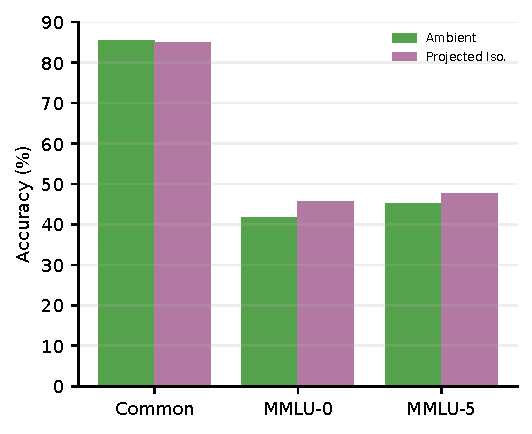
\includegraphics[width=\linewidth,trim=2mm 1mm 2mm 1mm,clip]
  {Figure/component_projection.pdf}
  \caption{Projection}
\end{subfigure}\hfill
\begin{subfigure}[t]{0.32\linewidth}
  \centering
  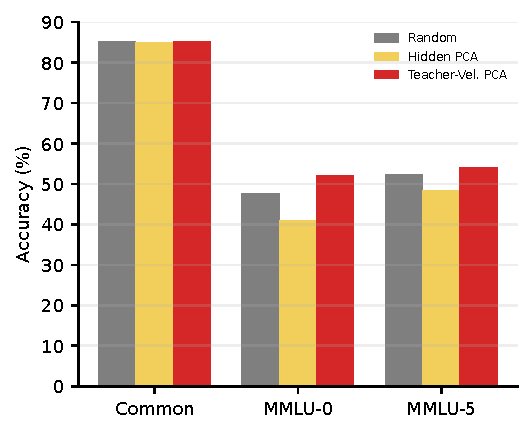
\includegraphics[width=\linewidth,trim=2mm 1mm 2mm 1mm,clip]
  {Figure/component_coordinates.pdf}
  \caption{Coordinate basis}
\end{subfigure}\hfill
\begin{subfigure}[t]{0.32\linewidth}
  \centering
  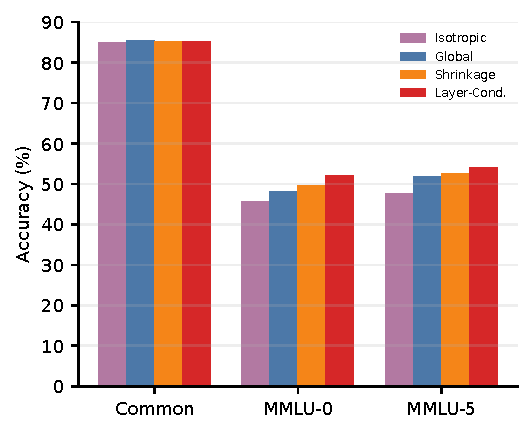
\includegraphics[width=\linewidth,trim=2mm 1mm 2mm 1mm,clip]
  {Figure/component_metrics.pdf}
  \caption{Within-subspace metric}
\end{subfigure}

\caption{\textbf{Matched component interventions.}
(a) Ambient versus projected isotropic velocity matching.
(b) Random, hidden-state-PCA, and teacher-velocity-PCA coordinates.
(c) Isotropic, global, shrinkage, and layer-conditioned metrics.
All settings use the same compressed architecture and report commonsense
and zero-/five-shot MMLU.}
\label{fig:component-interventions}
\end{figure}

Figure~\ref{fig:component-interventions} separates three questions that would be
confounded in the final FAD model.  First, replacing ambient matching by projected
isotropic matching changes commonsense by only $-0.50$ points but improves MMLU by
$+3.96/+2.54$ points, showing that restricting the recovery signal to a compact
subspace is useful.  Second, within a teacher-aware scaling protocol, the
teacher-velocity basis reaches $51.97/54.10$ MMLU, compared with $47.62/52.37$ for
a random subspace and $40.85/48.49$ for hidden-state PCA.  Random projection is
competitive, so the supported claim is not that arbitrary projection fails;
rather, projection supplies useful capacity allocation and teacher-velocity
coordinates give the strongest overall retention.  Third, within the fixed
velocity subspace, the layer-conditioned metric improves MMLU by $+6.24/+6.52$
points over isotropic matching, while global and shrinkage estimators lie between
the two.  Projection determines \emph{where} limited student capacity is spent,
whereas the teacher scale determines \emph{how} deviations inside that space are
priced.  Complete coordinate and metric tables are provided in
Appendix~\ref{app:geometry}.

The rank-$256$ teacher basis also remains concentrated beyond calibration: it
captures $45.20\%$ of held-out PIQA velocity energy versus $8.25\%$ for a random
subspace, and retains about a $2.5\times$ advantage on WikiText-2 and C4.  Because
PCA maximizes teacher variance by construction, this is a structural diagnostic;
Figure~\ref{fig:component-interventions} provides the causal downstream evidence,
and Appendix~\ref{tab:app-subspace-energy} reports the full values.

\subsection{Comparison with Structural Compression Baselines}
\label{sec:external-results}

\begin{table}[!t]
\caption{\textbf{External compression comparisons.}  Panel (a) reports the
seven-task commonsense macro at the nominal matched operating points used by the
separate 3B/8B study.  Panel (b) reports MMLU at the primary 3B operating point;
reductions are the exact values associated with each run.  Full per-task results
and accounting definitions are in Appendix~\ref{app:additional-results}.}
\label{tab:external-main}
\centering
\footnotesize
\renewcommand{\arraystretch}{1.02}
\setlength{\tabcolsep}{5.2pt}
\begin{tabular}{@{}llrrrr@{}}
\toprule
\multicolumn{6}{c}{\textbf{(a) Commonsense macro across backbones}}\\
\midrule
\textbf{Model} & \textbf{Compression rate} & \textbf{FLAP}
& \textbf{Tyr} & \textbf{Streamline} & \textbf{FAD}\\
\midrule
Llama-3.1-8B & 15\% & 79.83 & 83.61 & 86.86 & \textbf{87.67}\\
Llama-3.1-8B & 20\% & 76.99 & 81.72 & 86.87 & \textbf{87.66}\\
Llama-3.2-3B & 15\% & 70.59 & 79.30 & 81.29 & \textbf{85.38}\\
Llama-3.2-3B & 25\% & 63.89 & 72.71 & 81.25 & \textbf{85.03}\\
\midrule
\multicolumn{6}{c}{\textbf{(b) MMLU at the primary 3B point}}\\
\midrule
\multicolumn{2}{l}{\textbf{Method}} & \multicolumn{2}{c}{\textbf{Compression rate}}
& \textbf{0-shot} & \textbf{5-shot}\\
\midrule
\multicolumn{2}{l}{Dense teacher} & \multicolumn{2}{c}{0.00\%} & 49.42 & 51.20\\
\multicolumn{2}{l}{FLAP} & \multicolumn{2}{c}{20.05\%} & 35.29 & 36.36\\
\multicolumn{2}{l}{Tyr-the-Pruner} & \multicolumn{2}{c}{20.00\%} & 40.31 & 40.41\\
\multicolumn{2}{l}{LLM-Streamline} & \multicolumn{2}{c}{18.80\%} & 47.30 & 49.22\\
\multicolumn{2}{l}{\textbf{FAD}} & \multicolumn{2}{c}{\textbf{20.93\%}}
& \textbf{51.97} & \textbf{54.10}\\
\bottomrule
\end{tabular}
\end{table}

FAD has the highest commonsense macro at all four 3B/8B operating points in
Table~\ref{tab:external-main}(a).  The margin over LLM-Streamline is modest on 8B
($0.81/0.79$ points) and larger on 3B ($4.09/3.78$ points), indicating that the
recovery signal is especially useful under the tighter small-model bottleneck.
At the primary 3B point, FAD also exceeds LLM-Streamline by $4.67/4.88$ MMLU
points while using the larger reported reduction.  These comparisons complement,
rather than replace, the controlled objective study: the external table tests the
complete compression systems, whereas Table~\ref{tab:objective-main} isolates the
recovery signal.  The nominal 3B ``25\%'' row belongs to the external-baseline
experiment family and is not the controlled $K=17$ checkpoint used in the
compression stress test; the two rows must not be interpreted as repeated runs at
one exact reduction.

\subsection{Transport Fidelity under Recovery Objectives}
\label{sec:trajectory-results}

\begin{figure}[H]
\centering
\begin{subfigure}[t]{0.325\linewidth}
  \centering
  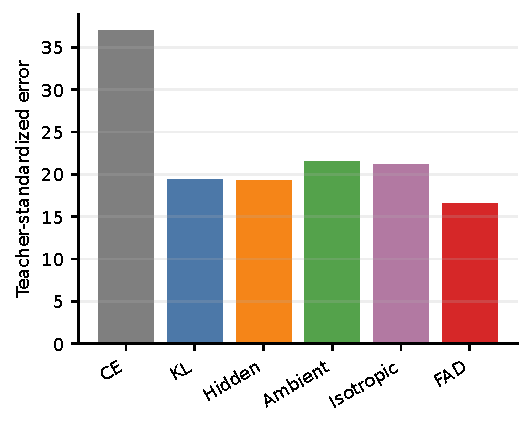
\includegraphics[width=\linewidth]{Figure/transport_teacher_metric.pdf}
  \caption{Teacher-standardized error $\downarrow$}
\end{subfigure}\hfill
\begin{subfigure}[t]{0.325\linewidth}
  \centering
  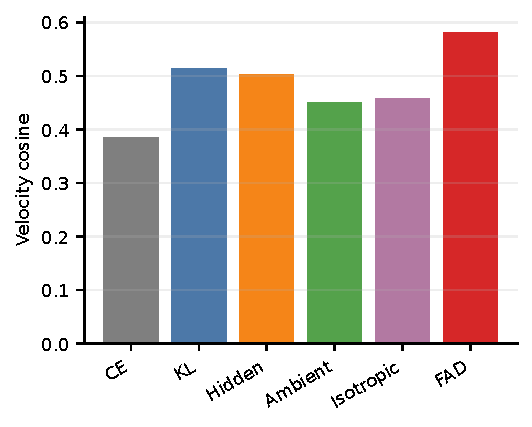
\includegraphics[width=\linewidth]{Figure/transport_cosine.pdf}
  \caption{Velocity cosine $\uparrow$}
\end{subfigure}\hfill
\begin{subfigure}[t]{0.325\linewidth}
  \centering
  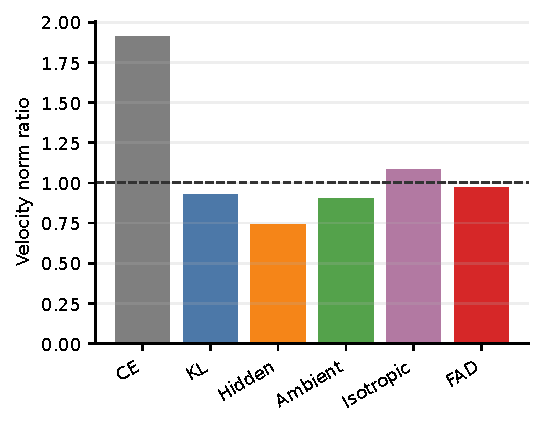
\includegraphics[width=\linewidth]{Figure/transport_norm_ratio.pdf}
  \caption{Norm ratio $\rightarrow 1$}
\end{subfigure}
\caption{\textbf{Held-out transport diagnostics on PIQA.}  FAD has the lowest
teacher-standardized transport error, the highest velocity cosine, and the norm
ratio closest to one.  Hidden-state MSE attains smaller raw state and ambient
velocity errors; the full diagnostic table is reported in Appendix~\ref{app:transport-diagnostics}.}
\label{fig:trajectory-core}
\end{figure}

Figure~\ref{fig:trajectory-core} connects the capability result to the quantity
FAD is designed to preserve.  Its advantage is not a generic reduction of every
Euclidean discrepancy: hidden-state matching has smaller raw state and ambient
velocity errors.  Instead, FAD most strongly preserves direction and magnitude in
the frozen teacher geometry, which is the selective transport-preservation claim
made by the method.  The directional cosine is not rescaled by the FAD precision
matrix and therefore provides a complementary check rather than merely restating
the optimized quadratic loss.

\subsection{Scope under Distribution Shift and Stronger Compression}
\label{sec:scope-results}

The task-aligned geometry does not preserve generic autoregressive likelihood to
the same degree: C4 NLL is $14.01$ for FAD, $2.76$ for the teacher, and $9.02$ for
logit KL.  Low-frequency C4 replay lowers FAD NLL to $6.40$ while retaining
$85.40$ commonsense and $52.82$ five-shot MMLU, but does not restore dense-model
likelihood.  Thus FAD is a \emph{task-aligned capability-preservation objective},
not a distribution-universal guarantee; Appendix~\ref{app:generic-lm} gives the
full analysis.

The advantage also narrows when structural capacity dominates.  At $25.58\%$ and
$30.23\%$ reduction, FAD remains strong for commonsense and relative to ambient
matching but is not the best MMLU objective.  Appendix~\ref{app:compression}
reports this stress test: recovery supervision cannot fully compensate for an
excessively restricted function class.

\subsection{Limitations}
\label{sec:limitations}

The central $K=19$ objective comparison uses three independently trained seeds per objective.  Evaluation-sample uncertainty is reported separately from training-seed variability.
We test
two Llama scales under one shared-FFN testbed.  The frozen geometry is
calibration-dependent and transfers incompletely to generic text.  Static sharing
reduces stored parameters but not logical depth; latency remains
implementation-dependent.

% ======================================================================
\section{Conclusion}
\label{sec:conclusion}
% ======================================================================

We studied which signal should be preserved after structural compression.
Across three independently trained seeds, competing recovery objectives achieve
similar in-domain commonsense accuracy, whereas FAD provides the strongest
average MMLU retention by aligning local FFN transport in teacher-derived
coordinates. Matched interventions isolate separate gains from projection,
velocity coordinates, and layer-conditioned scaling, while held-out diagnostics
confirm stronger directional and teacher-weighted transport fidelity. Gains
extend to 3B/8B structural baselines, while generic-text and high-compression
tests delimit the claim to task-aligned capability preservation.

% REQUIRED BEFORE SUBMISSION: insert the authors' verified AI Use Statement
% here, following the official ICLR 2027 policy.  Do not infer or fabricate it.

\subsection*{Reproducibility statement}
Section~\ref{sec:setup} defines the protocols.  Appendices
\ref{app:implementation}--\ref{app:generic-lm} provide provenance, accounting,
full results, and failure analyses; Appendix~\ref{app:grouping} fixes sharing;
and Appendices~\ref{app:maxent-derivation}--\ref{app:theory-properties} give the
complete derivations and theoretical scope.

\begingroup
\sloppy
\bibliography{reference}
\bibliographystyle{iclr2027_conference}
\endgroup

\clearpage
\appendix
\numberwithin{equation}{section}
\numberwithin{table}{section}
\numberwithin{figure}{section}

% Strict figure inclusion for the validated build: missing assets are fatal.

\noindent\textbf{Appendix organization.}
Appendix~\ref{app:implementation} specifies implementation and accounting;
Appendix~\ref{app:additional-results} gives full capability results;
Appendix~\ref{app:geometry} reports component and trajectory analyses;
Appendix~\ref{app:compression} studies stronger compression;
Appendix~\ref{app:generic-lm} diagnoses generic-language degradation;
Appendix~\ref{app:grouping} documents the fixed sharing construction;
Appendix~\ref{app:maxent-derivation} gives the complete variational derivation; and
Appendix~\ref{app:theory-properties} states the geometric, optimization, and
trajectory-stability results.

% ======================================================================
\section{Implementation and Reproducibility}
\label{app:implementation}
% ======================================================================

\subsection{Run Provenance}

The primary controlled study is locked to the Llama-3.2-3B $K=19$ bundle and its
frozen rank-$256$ velocity geometry.  The reported anchor is $51.97/54.10$ MMLU
under zero-/five-shot evaluation; these values are two protocols applied to the
same provenance-locked model, not independent retraining runs.  Internal run tags
are not used as model names in the paper.  The anonymous artifact should expose a
single immutable manifest containing the exact model and tokenizer revisions,
teacher checkpoint, geometry checksum, sharing assignment, adapter rank, optimizer
configuration, and evaluation commit.

\begin{table}[H]
\caption{Primary controlled-study identifiers and settings supported by the
reported results.  Low-level optimizer and checkpoint metadata are stored in the
submitted run manifest rather than reconstructed from prose.}
\label{tab:app-primary-config}
\centering
\small
\setlength{\tabcolsep}{7pt}
\renewcommand{\arraystretch}{1.04}
\begin{tabular}{@{}ll@{}}
\toprule
\textbf{Quantity} & \textbf{Primary value}\\
\midrule
Backbone & Llama-3.2-3B ($L=28$)\\
Stored FFN banks & $K=19$\\
Parameter reduction & $20.93\%$ of non-embedding model parameters\\
Projection variable & FFN residual velocity at the final valid context position\\
Projection rank & $r=256$\\
Private adapter rank & $\rho=128$\\
Training data & \texttt{commonsense\_170k}: $161{,}899/8{,}521$ train/validation\\
MMLU evaluator & \texttt{lm\_eval} v0.4.12, $14{,}042$ examples, 0-/5-shot\\
Evaluation seed & 44\\
Primary MMLU anchor & $51.97/54.10$\\
\bottomrule
\end{tabular}
\end{table}

\subsection{Teachers, Optimization, and Artifact Contract}

Each teacher is obtained by LoRA fine-tuning and merging.  To avoid silently
inventing run metadata, the exact LoRA targets, rank, scaling, dropout, base-model
revision, optimizer, learning-rate schedule, warmup, weight decay, gradient
clipping, effective batch size, sequence length, training steps, checkpoint rule,
FAD coefficient, coordinate grouping, stabilizer, and calibration size must be read
from the immutable anonymous configuration shipped with the corresponding row.
The artifact contract is one configuration and one result manifest per reported
model, together with frozen teacher geometry and scripts that regenerate all tables
and figures.  No table in this paper combines checkpoints whose bundle, geometry,
or evaluator provenance differs from its stated experiment family.

\subsection{Evaluation Protocol}

Commonsense evaluation uses log-probability multiple-choice scoring with one common
prompt and normalization protocol for all methods.  MMLU uses one task revision,
all $14{,}042$ questions, seed 44, and identical zero-/five-shot settings.  Geometry analyses use held-out examples and do not reuse training losses as
downstream metrics.  Any evaluation-example bootstrap interval must be reported
separately from variability across independently trained models.

\subsection{Compression Accounting}

We distinguish stored banks $K$, FFN-only reduction including adapters, exact
run-specific reduction, and rounded levels used only in the external 3B/8B study.
The primary $K=19$ point removes $20.93\%$ of non-embedding parameters, and
cross-family comparisons use exact reductions.

% ======================================================================
\clearpage
\section{Full Capability Results}
\label{app:additional-results}
% ======================================================================

\subsection{Full Structural-Baseline Breakdown}

\begin{table}[H]
\caption{\textbf{Seven-task matched-compression comparison.}  Values are
percent accuracy.  These nominal operating points belong to the separate external
compression study; they are not the controlled $K=19$ objective ablation.}
\label{tab:app-commonsense-full}
\centering
\scriptsize
\setlength{\tabcolsep}{2.8pt}
\renewcommand{\arraystretch}{1.03}
\resizebox{\linewidth}{!}{%
\begin{tabular}{@{}llrrrrrrrr@{}}
\toprule
\textbf{Method} & \textbf{Level} & \textbf{PIQA} & \textbf{SIQA}
& \textbf{Wino} & \textbf{ARC-C} & \textbf{ARC-E}
& \textbf{HellaS.} & \textbf{OBQA} & \textbf{Avg.}\\
\midrule
\multicolumn{10}{c}{\textbf{Llama-3.1-8B}}\\
\midrule
Dense teacher & -- & 88.57 & 79.79 & 83.66 & 80.38 & 90.91 & 95.45 & 84.40 & 86.17\\
FLAP & 15\% & 83.08 & 76.66 & 80.43 & 68.60 & 81.86 & 92.40 & 75.80 & 79.83\\
Tyr-the-Pruner & 15\% & 87.81 & 76.15 & 81.45 & 75.00 & 87.42 & 94.25 & 83.20 & 83.61\\
LLM-Streamline & 15\% & 89.28 & 79.53 & 86.03 & 80.12 & 91.79 & 95.87 & 85.40 & 86.86\\
\textbf{FAD} & 15\% & \textbf{89.72} & \textbf{80.66} & \textbf{86.35}
& \textbf{81.40} & \textbf{92.68} & \textbf{96.08} & \textbf{86.80} & \textbf{87.67}\\
\midrule
FLAP & 20\% & 81.39 & 75.74 & 75.37 & 64.76 & 77.36 & 90.88 & 73.40 & 76.99\\
Tyr-the-Pruner & 20\% & 86.89 & 75.95 & 79.79 & 71.67 & 84.89 & 93.22 & 79.60 & 81.72\\
LLM-Streamline & 20\% & 89.39 & 79.63 & 85.87 & 79.95 & 91.29 & 95.75 & \textbf{86.20} & 86.87\\
\textbf{FAD} & 20\% & \textbf{89.77} & \textbf{80.71} & \textbf{86.74}
& \textbf{81.66} & \textbf{92.72} & \textbf{96.00} & 86.00 & \textbf{87.66}\\
\midrule
\multicolumn{10}{c}{\textbf{Llama-3.2-3B}}\\
\midrule
Dense teacher & -- & 85.15 & 79.12 & 81.37 & 72.44 & 84.60 & 92.84 & 80.60 & 82.30\\
FLAP & 15\% & 78.51 & 72.06 & 66.46 & 55.29 & 69.70 & 85.34 & 66.80 & 70.59\\
Tyr-the-Pruner & 15\% & 83.41 & 76.31 & 77.58 & 67.41 & 80.72 & 90.49 & 79.20 & 79.30\\
LLM-Streamline & 15\% & 84.22 & 77.02 & 80.27 & 72.18 & 84.01 & 91.32 & 80.00 & 81.29\\
\textbf{FAD} & 15\% & \textbf{87.05} & \textbf{81.06} & \textbf{86.42}
& \textbf{76.28} & \textbf{87.50} & \textbf{94.55} & \textbf{84.80} & \textbf{85.38}\\
\midrule
FLAP & 25\% & 72.96 & 69.04 & 62.75 & 47.70 & 57.70 & 77.90 & 59.20 & 63.89\\
Tyr-the-Pruner & 25\% & 78.62 & 72.42 & 71.27 & 57.25 & 71.84 & 84.98 & 72.60 & 72.71\\
LLM-Streamline & 25\% & 83.90 & 76.61 & 80.35 & 71.93 & 84.64 & 91.91 & 79.40 & 81.25\\
\textbf{FAD} & 25\% & \textbf{85.96} & \textbf{79.02} & \textbf{86.74}
& \textbf{77.30} & \textbf{88.68} & \textbf{94.12} & \textbf{83.40} & \textbf{85.03}\\
\bottomrule
\end{tabular}%
}
\end{table}

\subsection{MMLU Domains under Controlled Objectives}
\label{app:mmlu-domains-objectives}

\begin{table}[H]
\caption{MMLU domain accuracy for the controlled $K=19$ objective study.  Each
cell is zero-shot / five-shot.  FAD is best in every domain and protocol.}
\label{tab:app-objective-domains}
\centering
\footnotesize
\setlength{\tabcolsep}{4.2pt}
\renewcommand{\arraystretch}{1.04}
\begin{tabular}{@{}lccccc@{}}
\toprule
\textbf{Objective} & \textbf{Humanities} & \textbf{Other}
& \textbf{Social Sci.} & \textbf{STEM} & \textbf{Overall}\\
\midrule
CE only & 27.84/30.52 & 26.39/30.00 & 27.07/33.18 & 28.96/32.89 & 27.60/31.52\\
Logit KL & 34.81/36.81 & 46.99/50.31 & 47.64/49.66 & 36.63/38.50 & 40.73/42.99\\
Hidden MSE & 39.64/41.68 & 52.85/53.88 & 53.01/55.74 & 40.66/42.50 & 45.72/47.64\\
Ambient & 36.90/40.45 & 47.34/51.14 & 47.29/51.84 & 38.19/39.26 & 41.77/45.04\\
Isotropic & 41.87/43.04 & 50.53/52.66 & 53.56/56.19 & 39.14/40.95 & 45.73/47.58\\
\textbf{FAD} & \textbf{46.31/49.76} & \textbf{58.64/59.64}
& \textbf{61.88/63.44} & \textbf{44.15/46.02} & \textbf{51.97/54.10}\\
\bottomrule
\end{tabular}
\end{table}

Table~\ref{tab:mmlu-domain-consistency} summarizes the strongest alternative
in each domain.  This full matrix shows which objective supplies that alternative
and confirms that the overall gain is not driven by one domain.

\subsection{MMLU Domains against Structural Baselines}

\begin{table}[H]
\centering
\begin{subtable}[t]{0.48\linewidth}
\centering\footnotesize
\caption{0-shot}
\label{tab:app-mmlu-zero-domain}
\setlength{\tabcolsep}{3.1pt}
\begin{tabular}{@{}lrrrr@{}}
\toprule
\textbf{Method} & \textbf{STEM} & \textbf{Hum.} & \textbf{Social} & \textbf{Other}\\
\midrule
FAD & \textbf{44.15} & \textbf{46.31} & \textbf{61.88} & \textbf{58.64}\\
Streamline & 38.66 & 43.95 & 53.92 & 54.59\\
Tyr & 34.92 & 37.41 & 44.07 & 46.44\\
FLAP & 32.13 & 32.65 & 38.64 & 39.20\\
\bottomrule
\end{tabular}
\end{subtable}\hfill
\begin{subtable}[t]{0.48\linewidth}
\centering\footnotesize
\caption{5-shot}
\label{tab:app-mmlu-five-domain}
\setlength{\tabcolsep}{3.1pt}
\begin{tabular}{@{}lrrrr@{}}
\toprule
\textbf{Method} & \textbf{STEM} & \textbf{Hum.} & \textbf{Social} & \textbf{Other}\\
\midrule
FAD & \textbf{46.02} & \textbf{49.76} & \textbf{63.44} & \textbf{59.64}\\
Streamline & 41.33 & 44.44 & 56.68 & 57.06\\
Tyr & 35.65 & 36.81 & 46.15 & 45.00\\
FLAP & 32.98 & 33.50 & 40.10 & 40.39\\
\bottomrule
\end{tabular}
\end{subtable}
\caption{MMLU domain-level accuracy against structural compression baselines.}
\label{tab:app-mmlu-domains-structural}
\end{table}

\subsection{Training-Seed Evidence}

\begin{table}[H]
\caption{Multi-seed results for FAD at the primary operating point. Values
report three independently trained seeds and their mean $\pm$ sample standard
deviation.}
\label{tab:app-seeds}
\centering
\small
\setlength{\tabcolsep}{8pt}
\begin{tabular}{@{}lccc@{}}
\toprule
\textbf{Seed} & \textbf{Commonsense macro}
& \textbf{MMLU 0-shot} & \textbf{MMLU 5-shot}\\
\midrule
42 & 84.47 & 44.99 & 50.19\\
43 & 84.76 & 45.70 & 51.99\\
44 & 85.30 & 51.97 & 54.10\\
\midrule
Mean $\pm$ sample std.
& $84.84\pm0.42$
& $47.55\pm3.84$
& $52.09\pm1.96$\\
\bottomrule
\end{tabular}
\end{table}

% The disputed paired-seed MMLU figure is intentionally excluded.  It may be
% restored only after a provenance-aligned seed audit confirms that every run
% uses the primary bundle definition and evaluator.

% ======================================================================
\FloatBarrier
\section{Component, Geometry, and Trajectory Analyses}
\label{app:geometry}
% ======================================================================

\subsection{Coordinate and Metric Controls}
\label{app:coordinate-controls}

\begin{table}[H]
\centering
\begin{subtable}[t]{0.49\linewidth}
\centering\footnotesize
\caption{Coordinate basis with teacher-aware scaling}
\label{tab:app-coordinate-controls}
\setlength{\tabcolsep}{3.4pt}
\begin{tabular}{@{}lrrr@{}}
\toprule
\textbf{Basis} & \textbf{Common.} & \textbf{M0} & \textbf{M5}\\
\midrule
Random subspace & 85.28 & 47.62 & 52.37\\
Hidden-state PCA & 85.01 & 40.85 & 48.49\\
\textbf{Velocity PCA} & \textbf{85.30} & \textbf{51.97} & \textbf{54.10}\\
\bottomrule
\end{tabular}
\end{subtable}\hfill
\begin{subtable}[t]{0.49\linewidth}
\centering\footnotesize
\caption{Metric inside velocity PCA}
\label{tab:app-metric-controls}
\setlength{\tabcolsep}{3.4pt}
\begin{tabular}{@{}lrrr@{}}
\toprule
\textbf{Metric} & \textbf{Common.} & \textbf{M0} & \textbf{M5}\\
\midrule
Isotropic & 85.03 & 45.73 & 47.58\\
Global teacher & 85.38 & 48.22 & 51.83\\
Shrinkage teacher & 85.31 & 49.60 & 52.66\\
\textbf{Layer-conditioned} & 85.30 & \textbf{51.97} & \textbf{54.10}\\
\bottomrule
\end{tabular}
\end{subtable}
\caption{Coordinate and metric controls at the primary operating point.  Random
projection is competitive, so the supported claim is that projection itself is
useful and teacher-velocity coordinates with layer conditioning give the best
overall retention--not that every random projection fails.}
\label{tab:app-coordinate-metric-controls}
\end{table}

\begin{table}[H]
\caption{Held-out energy captured by the rank-$256$ teacher-velocity PCA basis
and a random subspace of the same rank.  This table establishes persistent
low-rank teacher structure; downstream causality is tested by the matched
interventions in Figure~\ref{fig:component-interventions}.}
\label{tab:app-subspace-energy}
\centering
\small
\setlength{\tabcolsep}{9pt}
\renewcommand{\arraystretch}{1.04}
\begin{tabular}{@{}lrrr@{}}
\toprule
\textbf{Held-out data} & \textbf{Teacher PCA} & \textbf{Random} & \textbf{Ratio}\\
\midrule
PIQA & \textbf{45.20\%} & 8.25\% & $5.48\times$\\
WikiText-2 & \textbf{20.83\%} & 8.30\% & $2.51\times$\\
C4 & \textbf{20.42\%} & 8.30\% & $2.46\times$\\
\bottomrule
\end{tabular}
\end{table}

\subsection{Complete Transport Diagnostics}
\label{app:transport-diagnostics}

\begin{table}[H]
\caption{Aggregate held-out PIQA diagnostics corresponding to
Figure~\ref{fig:trajectory-core}.  Final $d_h$ is measured at the last block; the
remaining quantities are averaged over the evaluated transport layers.}
\label{tab:app-transport-diagnostics}
\centering
\footnotesize
\setlength{\tabcolsep}{4.3pt}
\renewcommand{\arraystretch}{1.04}
\begin{tabular}{@{}lccccc@{}}
\toprule
\textbf{Recovery objective} & \textbf{Final $d_h$ $\downarrow$}
& \textbf{Mean $d_v$ $\downarrow$} & \textbf{Teacher error $\downarrow$}
& \textbf{Cosine $\uparrow$} & \textbf{Norm ratio $\to1$}\\
\midrule
Hidden-state MSE & \textbf{77.08} & \textbf{5.79} & 19.33 & 0.503 & 0.739\\
Ambient velocity MSE & 90.65 & 6.63 & 21.53 & 0.450 & 0.901\\
\textbf{FAD} & 84.64 & 6.97 & \textbf{16.60} & \textbf{0.581} & \textbf{0.972}\\
\bottomrule
\end{tabular}
\end{table}

The diagnostics separate raw Euclidean matching from teacher-weighted transport
preservation.  Hidden-state MSE minimizes final-state and ambient-velocity error,
whereas FAD produces the lowest teacher-standardized error, strongest directional
agreement, and most accurate update magnitude.  This distinction prevents the
mechanistic analysis from claiming universal dominance over every discrepancy.

\subsection{Projection Rank and Calibration Sensitivity}

\begin{table}[H]
\centering
\begin{subtable}[t]{0.49\linewidth}
\centering\footnotesize
\caption{Projection rank}
\label{tab:app-projection-rank}
\setlength{\tabcolsep}{4pt}
\begin{tabular}{@{}rrrr@{}}
\toprule
$r$ & \textbf{Common.} & \textbf{M0} & \textbf{M5}\\
\midrule
32 & 85.13 & 37.38 & 43.07\\
64 & 85.24 & 43.95 & 50.31\\
128 & \textbf{85.57} & 46.40 & 49.22\\
256 & 85.30 & \textbf{51.97} & \textbf{54.10}\\
\bottomrule
\end{tabular}
\end{subtable}\hfill
\begin{subtable}[t]{0.47\linewidth}
\centering\footnotesize
\caption{Geometry calibration}
\label{tab:app-calibration}
\setlength{\tabcolsep}{5pt}
\begin{tabular}{@{}lc@{}}
\toprule
\textbf{Setting} & \textbf{Commonsense}\\
\midrule
1k examples & 85.21\\
4k examples & 85.32\\
16k examples & \textbf{85.47}\\
Full, seed 42 & 85.40\\
Full, seed 43 & 85.22\\
Full, seed 44 & 85.30\\
\bottomrule
\end{tabular}
\end{subtable}
\caption{Projection-rank and calibration sensitivity.  MMLU is not monotone in
rank, so the supported statement is that $r=256$ is best among the tested ranks,
not that larger rank is guaranteed to improve performance.}
\label{tab:app-rank-calibration}
\end{table}

\subsection{Teacher Scale}

The diagonal teacher scale ranges from approximately $8.0\times10^{-5}$ to $74.8$
(about $5.97$ orders of magnitude), with layer-wise condition numbers from roughly
$82$ to $3{,}845$.  This anisotropy motivates layer-wise standardization; the
matched metric intervention in the main text establishes its downstream
contribution.

\begin{figure}[H] \centering \begin{subfigure}[t]{0.49\linewidth} \centering 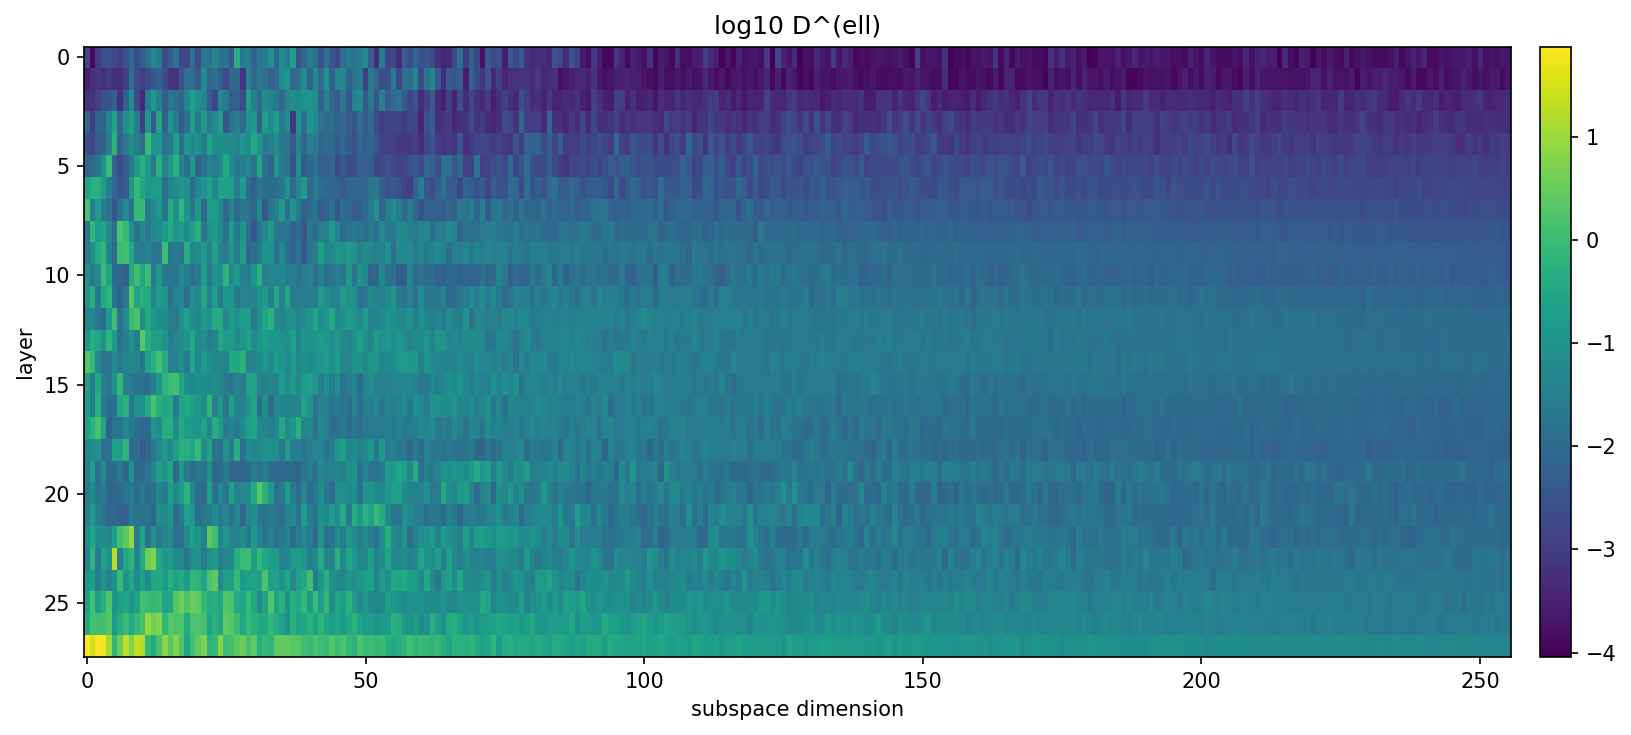
\includegraphics[width=\linewidth]{Figure/teacher_scale_D_log_heatmap.png} \caption{Teacher scale} \end{subfigure}\hfill \begin{subfigure}[t]{0.49\linewidth} \centering 
\includegraphics[width=\linewidth]{Figure/teacher_scale_inv_std_heatmap.png} \caption{Whitening weights} \end{subfigure} \caption{Layer-by-direction teacher scale and corresponding standardization weights with identical ordering. The broad range motivates direction-dependent normalization; Figure~\ref{fig:component-interventions}(c) tests its downstream contribution.} \label{fig:app-teacher-geometry} \end{figure}



% ======================================================================
\FloatBarrier
\section{Compression-Regime Robustness}
\label{app:compression}
% ======================================================================

\subsection{Objective Comparison under Stronger Compression}

\begin{table}[H]
\caption{Controlled recovery objectives across compression regimes.  Best values
within each $K$ block are bold.}
\label{tab:app-compression-objectives}
\centering
\footnotesize
\setlength{\tabcolsep}{5pt}
\begin{tabular}{@{}rrlrrr@{}}
\toprule
$K$ & \textbf{Reduction} & \textbf{Objective} & \textbf{Common.}
& \textbf{MMLU-0} & \textbf{MMLU-5}\\
\midrule
19 & 20.93\% & Logit KL & 84.97 & 40.73 & 42.99\\
19 & 20.93\% & Hidden MSE & 84.98 & 45.72 & 47.64\\
19 & 20.93\% & Ambient & \textbf{85.53} & 41.77 & 45.04\\
19 & 20.93\% & Isotropic & 85.03 & 45.73 & 47.58\\
19 & 20.93\% & \textbf{FAD} & 85.30 & \textbf{51.97} & \textbf{54.10}\\
\midrule
17 & 25.58\% & Logit KL & 77.37 & 36.36 & \textbf{39.02}\\
17 & 25.58\% & Hidden MSE & 77.74 & \textbf{38.63} & 36.38\\
17 & 25.58\% & Ambient & 76.31 & 30.12 & 27.15\\
17 & 25.58\% & Isotropic & 77.36 & 30.27 & 31.23\\
17 & 25.58\% & \textbf{FAD} & \textbf{78.69} & 37.46 & 31.95\\
\midrule
15 & 30.23\% & Logit KL & 71.11 & \textbf{28.85} & \textbf{31.49}\\
15 & 30.23\% & Hidden MSE & 70.01 & 28.27 & 29.25\\
15 & 30.23\% & Ambient & 67.87 & 23.24 & 23.04\\
15 & 30.23\% & Isotropic & 71.81 & 28.78 & 29.08\\
15 & 30.23\% & \textbf{FAD} & \textbf{73.32} & 26.88 & 28.44\\
\bottomrule
\end{tabular}
\end{table}

FAD has the strongest commonsense recovery at $K=17$ and $K=15$ and remains
substantially better than ambient matching.  It is not the strongest MMLU objective
in these aggressively compressed regimes, and the absolute $K=15$ MMLU score is
near the lower end of the evaluation range.  These results support robustness to
ambient matching, not a claim that FAD dominates every objective at every capacity.

\begin{figure}[H]
\centering
\begin{subfigure}[t]{0.325\linewidth}
  \centering
  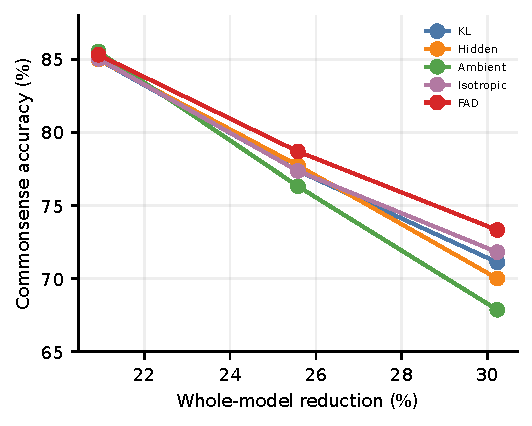
\includegraphics[width=\linewidth]{Figure/compression_commonsense.pdf}
  \caption{Commonsense}
\end{subfigure}\hfill
\begin{subfigure}[t]{0.325\linewidth}
  \centering
  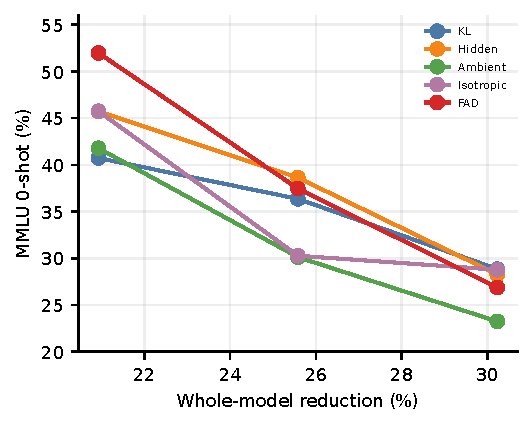
\includegraphics[width=\linewidth]{Figure/compression_mmlu0.pdf}
  \caption{MMLU 0-shot}
\end{subfigure}\hfill
\begin{subfigure}[t]{0.325\linewidth}
  \centering
  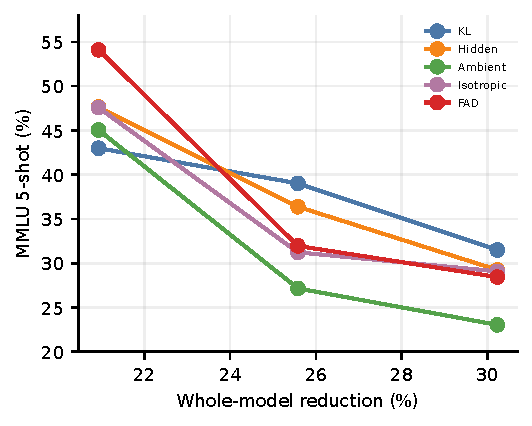
\includegraphics[width=\linewidth]{Figure/compression_mmlu5.pdf}
  \caption{MMLU 5-shot}
\end{subfigure}
\caption{Controlled objectives under stronger structural compression.  The
primary claim is anchored at $K=19$; $K=17/15$ expose the capacity-limited regime.}
\label{fig:app-compression-curves}
\end{figure}

\subsection{Nested Structural Restriction}

For fixed teacher geometry and a refinement sequence of sharing partitions,
Theorem~\ref{thm:app-nested-classes} orders the global optima of the nested model
classes.  The observed FAD loss rises from $0.104$ to $0.176$ as exact reduction
increases from $13.95\%$ to $30.23\%$ for $K=22,19,17,15$.

\begin{figure}[H]
\centering
\begin{subfigure}[t]{0.49\linewidth}
  \centering
  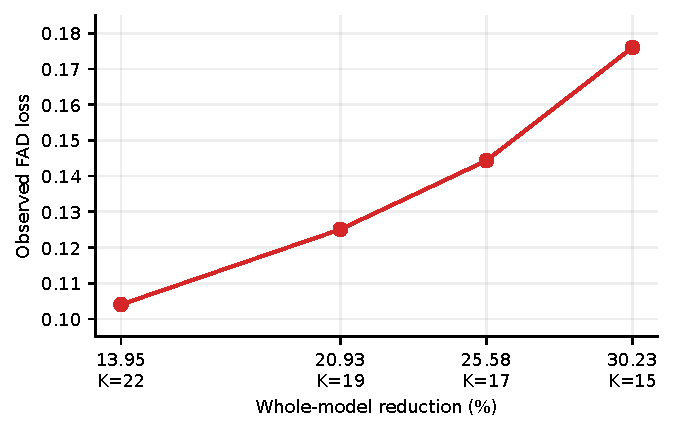
\includegraphics[width=\linewidth]{Figure/nested_fad_loss.pdf}
  \caption{Observed FAD loss}
\end{subfigure}\hfill
\begin{subfigure}[t]{0.49\linewidth}
  \centering
  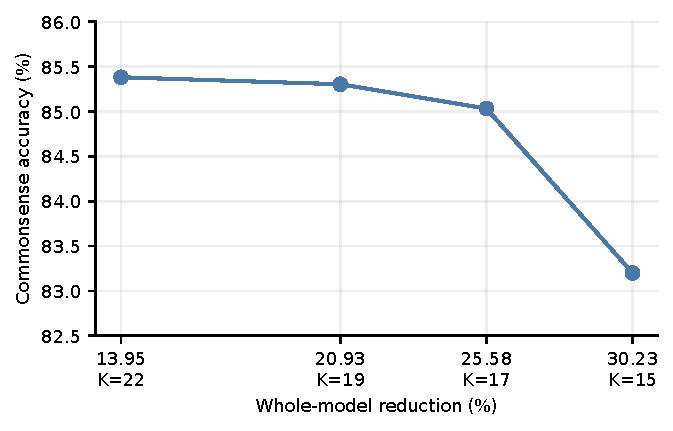
\includegraphics[width=\linewidth]{Figure/nested_commonsense.pdf}
  \caption{Commonsense accuracy}
\end{subfigure}
\caption{Nested structural restriction and observed transport distortion.  The
monotone trained losses support the nested-class prediction but do not prove
convergence of the nonconvex CE--FAD training problem.}
\label{fig:app-nested-information}
\end{figure}

% ======================================================================
\FloatBarrier
\section{Generic-Language Trade-off and Mitigation}
\label{app:generic-lm}
% ======================================================================

\subsection{Evaluator Sanity Check}

\begin{table}[H]
\caption{Uncompressed generic-language likelihood verifies that the evaluator is
operating in a normal range before structural recovery.}
\label{tab:app-generic-sanity}
\centering
\small
\setlength{\tabcolsep}{9pt}
\begin{tabular}{@{}lrrrr@{}}
\toprule
\textbf{Model} & \textbf{Wiki NLL} & \textbf{Wiki PPL}
& \textbf{C4 NLL} & \textbf{C4 PPL}\\
\midrule
Base model & 2.233 & 9.33 & 2.456 & 11.66\\
Teacher & 2.518 & 12.41 & 2.760 & 15.80\\
\bottomrule
\end{tabular}
\end{table}

\subsection{Generic-Language Degradation by Objective}

\begin{table}[H]
\caption{C4 likelihood under the controlled recovery objectives.  Lower is
better.  All structurally recovered variants degrade, while all-token logit KL is
the least affected.}
\label{tab:app-c4-objectives}
\centering
\small
\setlength{\tabcolsep}{10pt}
\begin{tabular}{@{}lrr@{}}
\toprule
\textbf{Objective} & \textbf{C4 NLL} & \textbf{C4 PPL}\\
\midrule
CE only & 15.963 & 8,566,947\\
Logit KL & \textbf{9.024} & \textbf{8,298}\\
Hidden MSE & 12.030 & 167,631\\
Ambient & 13.535 & 755,494\\
Isotropic & 14.091 & 1,316,761\\
FAD & 14.011 & 1,215,258\\
\bottomrule
\end{tabular}
\end{table}

The recovery data emphasize commonsense decisions and the aligned signal is read at
the final prediction position, so generic all-token language modeling is
underconstrained.  The result is not unique to FAD, but it rules out a universal
language-model preservation claim.

\subsection{Low-Frequency Generic Replay}

\begin{table}[H]
\caption{Mitigating the generic-language trade-off.  Mild C4 replay gives the best
observed balance, but remains far from the uncompressed likelihood.}
\label{tab:app-c4-remedies}
\centering
\footnotesize
\setlength{\tabcolsep}{4.5pt}
\begin{tabular}{@{}lrrrrrr@{}}
\toprule
\textbf{Variant} & \textbf{Common.} & \textbf{M0} & \textbf{M5}
& \textbf{Wiki NLL} & \textbf{C4 NLL} & \textbf{C4 PPL}\\
\midrule
FAD anchor & 85.30 & \textbf{51.97} & \textbf{54.10} & 13.121 & 14.011 & 1,215,258\\
FAD + KL(.25) & 85.07 & 41.34 & 52.07 & 10.149 & 10.574 & 39,111\\
\textbf{FAD + mild replay (1/10)} & \textbf{85.40} & 47.22 & 52.82
& \textbf{6.687} & \textbf{6.398} & \textbf{600.8}\\
FAD + strong replay (1/4) & 85.27 & 45.64 & 52.67 & 7.534 & 7.189 & 1,324.6\\
FAD + KL + replay & 84.87 & 41.61 & 52.08 & 7.375 & 7.474 & 1,761.9\\
\bottomrule
\end{tabular}
\end{table}

Mild replay lowers C4 NLL by $7.61$ ($54.3\%$), leaves commonsense unchanged, and
retains $52.82$ five-shot MMLU.  Its C4 perplexity remains much higher than the
base model and teacher, and the remedy evidence is currently single-seed.

\begin{figure}[H]
\centering
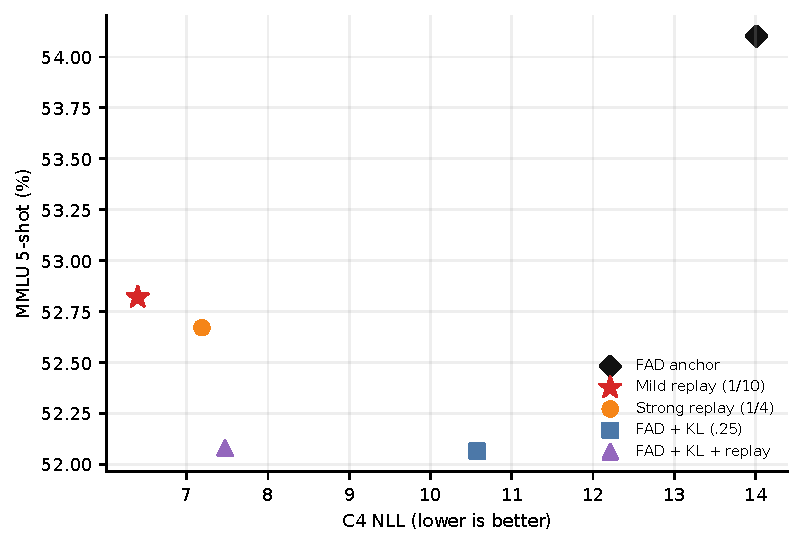
\includegraphics[width=0.88\linewidth]{Figure/c4_mmlu_pareto_revised.pdf}
\caption{\textbf{Generic-language trade-off under replay mitigation.}
Low-frequency C4 replay substantially reduces generic-language NLL while
retaining most of the five-shot MMLU performance.}
\label{fig:app-generic-tradeoff}
\end{figure}

\FloatBarrier
\section{Functional Sharing Construction}
\label{app:grouping}
% ======================================================================


\subsection{Fixed-Budget Assignment Control}
\label{app:sharing-control}

\begin{table}[H]
\caption{Sharing-policy comparison at fixed $K=19$ capacity.  The recovery
objective, seed, and evaluation protocol are fixed; only the assignment changes.}
\label{tab:app-sharing-policy}
\centering
\small
\setlength{\tabcolsep}{10pt}
\begin{tabular}{@{}lcc@{}}
\toprule
\textbf{Sharing policy} & \textbf{$K$} & \textbf{Commonsense macro}\\
\midrule
\textbf{Restricted-late} & 19 & \textbf{85.30}\\
Random & 19 & 82.52\\
Unrestricted complete-link & 19 & 80.36\\
Same-regime complete-link & 19 & 80.32\\
Adjacent grouping & 19 & 65.74\\
\bottomrule
\end{tabular}
\end{table}

At fixed capacity, assignment choice materially affects recovery.  This table is a
control for the structural testbed, not a second main contribution: all controlled
objective comparisons in the paper freeze the same restricted-late assignment.

\subsection{Replacement Cost}
For an admissible pair $(\ell,\ell')$, temporarily replace the FFN at layer
$\ell'$ with that at layer $\ell$ while keeping the remaining model fixed:
\begin{equation}
  C_{\ell\to\ell'}
  = \Delta\NLL_{\ell\to\ell'}
  + \lambda_{\KL}D_{\KL}\!\left(p_{\mathrm{base}}\,\|\,
  p_{\ell\to\ell'}\right),\qquad \lambda_{\KL}=1.
  \label{eq:app-replacement-cost}
\end{equation}
The symmetric cost uses the worse direction,
\begin{equation}
  C^{\mathrm{bi}}_{\ell\ell'}
  =\max\!\left(C_{\ell\to\ell'},C_{\ell'\to\ell}\right).
  \label{eq:app-bidirectional-cost}
\end{equation}
Complete-link merging controls the largest cross-pair cost; restricted-late
sharing additionally applies the admissibility mask used by the primary run.

% ----------------------------------------------------------------------
% [ADDED-THEORY-B1] What complete-link controls and what the pairwise
% replacement surrogate does not guarantee.
\subsection{Complete-Link Criterion and Its Scope}
\label{app:complete-link-scope}
% ----------------------------------------------------------------------

For two current clusters $A$ and $B$, complete-link agglomeration uses
\begin{equation}
  d_{\mathrm{CL}}(A,B)
  =\max_{\ell\in A,\,\ell'\in B}C^{\mathrm{bi}}_{\ell\ell'}.
  \label{eq:app-complete-link-distance}
\end{equation}
After merging $A$ and $B$, the diameter of the resulting cluster $G=A\cup B$ is
\begin{equation}
  \operatorname{diam}_{C}(G)
  =\max_{i,j\in G}C^{\mathrm{bi}}_{ij}.
  \label{eq:app-cluster-diameter}
\end{equation}
Thus complete-link directly tracks a worst observed pairwise replacement cost,
rather than an average pairwise cost.  Cutting the hierarchy at a merge height
$\tau$ produces clusters whose pairwise diameter does not exceed $\tau$ among the
admissible pairs represented in the hierarchy.  This is the formal reason for
using complete-link when a single high-cost pairing inside a shared group is
undesirable.

The guarantee is limited to the measured surrogate.  Each
$C_{\ell\to\ell'}$ is obtained by replacing one layer while the remainder of the
model is fixed.  Simultaneously sharing several layers can create interaction
terms that are absent from all single-replacement measurements.  Therefore
Eq.~\eqref{eq:app-cluster-diameter} does not upper-bound the end-to-end degradation
of the final multi-layer shared model without an additional additivity or
stability assumption.  The fixed-budget assignment control in Appendix~\ref{app:sharing-control} is the
empirical validation of this surrogate.

% BLOCKING REPRODUCIBILITY ITEM (not printed): the anonymous manifest must specify
% the medoid objective and deterministic tie-breaking rule. The available source
% does not contain this information, so it is not invented here.


\subsection{Nested Assignments}
All unlisted layers remain private:
\begin{align*}
K=22:&\quad \{19,\ldots,24\},\ \{25,26\},\\
K=19:&\quad \{16,17,18\},\ \{19,\ldots,26\},\\
K=17:&\quad \{14,\ldots,18\},\ \{19,\ldots,26\},\\
K=15:&\quad \{12,\ldots,18\},\ \{19,\ldots,26\}.
\end{align*}
These assignments satisfy the refinement condition used by
Theorem~\ref{thm:app-nested-classes}.

\begin{figure}[H]
\centering
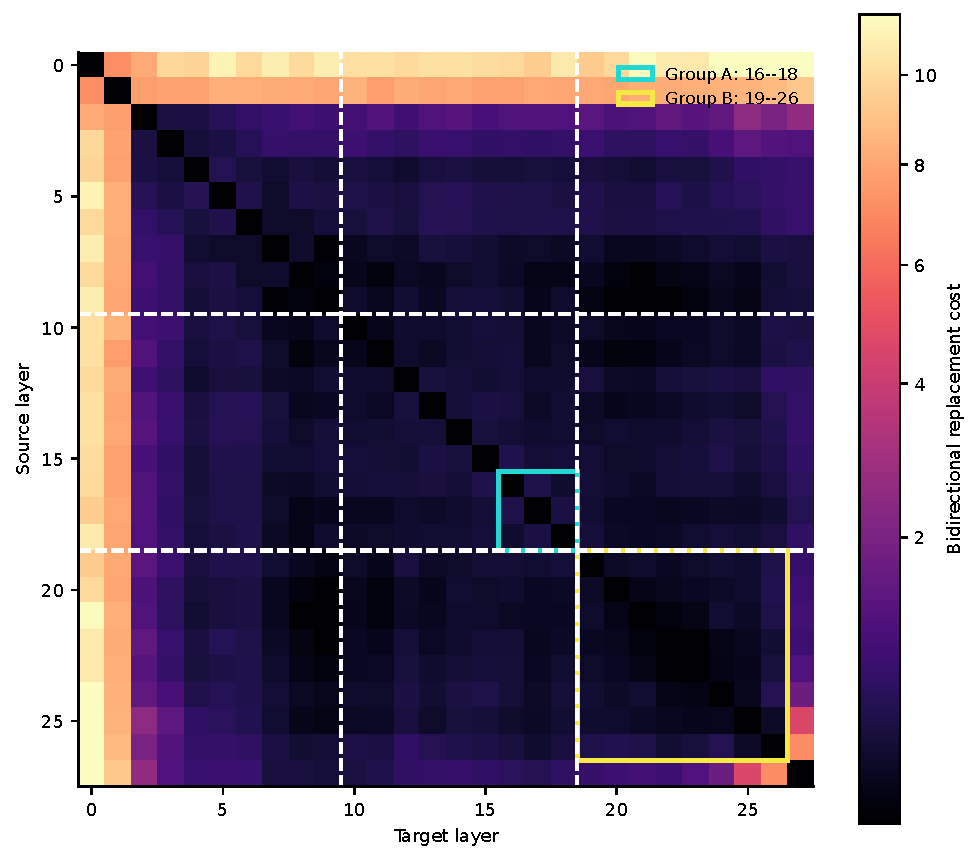
\includegraphics[width=0.72\linewidth]{Figure/replacement_cost_heatmap.pdf}
\caption{\textbf{Replacement-cost geometry.}  The bidirectional cost matrix
$C^{\mathrm{bi}}_{\ell\ell'}$ is shown with depth boundaries and the primary
$K=19$ restricted-late groups overlaid.}
\label{fig:app-replacement}
\end{figure}

\subsection{Initialization and Private Adapters}
Each shared bank is initialized from its policy medoid. The private adapter is
zero-initialized so that step zero isolates the mismatch introduced by sharing.
Appendix~\ref{app:geometry} reports calibration, projection-rank, and
initialization sensitivity.

% ----------------------------------------------------------------------
% [ADDED-THEORY-B2] Expressivity and initialization of the private low-rank
% correction.
\subsection{Capacity and Initialization of the Private Adapter}
\label{app:adapter-capacity-theory}
% ----------------------------------------------------------------------

For a fixed layer and a batch of normalized FFN inputs collected as columns of
$X_\ell\in\R^{D\times N}$, the private adapter produces
\begin{equation}
  Y_{\mathrm{ad}}^{(\ell)}=U^{(\ell)}V^{(\ell)}X_\ell.
  \label{eq:app-adapter-batch-output}
\end{equation}
Its batch output satisfies
\begin{equation}
  \operatorname{rank}(Y_{\mathrm{ad}}^{(\ell)})
  \le\min\!\left\{\rho,\operatorname{rank}(X_\ell),N\right\}.
  \label{eq:app-adapter-rank-bound}
\end{equation}
Hence the adapter can supply at most a rank-$\rho$ linear correction on a fixed
batch.  This is an expressivity statement about the correction branch; FAD
supervises the sum of the shared branch and the adapter and does not require the
two contributions to be identifiable.

With $U^{(\ell)}=0$ and a nonzero initialization of $V^{(\ell)}$, the adapter
output is exactly zero at step zero, while gradients can first update
$U^{(\ell)}$.  If both factors are initialized to zero, then the first-step
gradients of both factors are zero:
\begin{equation}
  \frac{\partial\calL}{\partial U}
  =G(VX)^\top=0,
  \qquad
  \frac{\partial\calL}{\partial V}
  =U^\top GX^\top=0,
  \label{eq:app-double-zero-gradient}
\end{equation}
where $G$ is the upstream gradient.  The artifact must therefore record the
initialization of both $U^{(\ell)}$ and $V^{(\ell)}$, not only the fact that the
adapter output begins at zero.


% ======================================================================
% [ADDED-THEORY-C0] Complete derivation of the variational information
% objective, its maximum-entropy inner problem, and its exact reduction to
% the implemented FAD loss.
% ======================================================================
\clearpage
\section{Complete Information-Preservation Derivation}
\label{app:maxent-derivation}
% ======================================================================

This appendix states the population variables, the variational objective, the
measure under which the conditional density is defined, the complete
maximum-entropy calculation, and the precise assumptions under which the
implemented FAD loss is equivalent to maximizing a variational mutual-information
lower bound.  It also separates three choices that play different roles:
(i) the FFN residual update is the aligned variable; (ii) teacher PCA selects the
modeled coordinates; and (iii) the teacher scale matrix specifies the conditional
uncertainty used by the variational surrogate.  The maximum-entropy argument
solves the conditional model only after these choices have been fixed.

% ----------------------------------------------------------------------
\subsection{Population Variables and a Well-Defined Conditional Density}
\label{app:population-formulation}
% ----------------------------------------------------------------------

Let $X\sim P_X$ denote a random training example, including the token position at
which the velocities are extracted.  For a fixed supervised layer $\ell$, define
the projected teacher and student random variables
\begin{equation}
  \boldsymbol{Z}_T^{(\ell)}=\bz_T^{(\ell)}(X),
  \qquad
  \boldsymbol{Z}_{S,\theta}^{(\ell)}=\bz_S^{(\ell)}(X;\theta),
  \qquad \theta\in\Theta_{\mathrm{shared}}.
  \label{eq:app-population-codes}
\end{equation}
The teacher, projection basis, centering vector, and scale matrix are fixed;
only the student random variable depends on $\theta$.

Because language-model inputs are discrete and both networks are deterministic,
the induced distributions can be atomic.  Writing a differential entropy and a
Lebesgue density for such variables without qualification can therefore create a
base-measure mismatch.  We make the variational statement rigorous by introducing
an arbitrarily small, student-independent smoothing of the teacher code,
\begin{equation}
  \widetilde{\boldsymbol{Z}}_{T,\tau}^{(\ell)}
  =\boldsymbol{Z}_T^{(\ell)}+\tau\boldsymbol{\varepsilon},
  \qquad
  \boldsymbol{\varepsilon}\sim\calN(\boldsymbol{0},\bI_r),
  \qquad \tau>0,
  \label{eq:app-smoothed-teacher}
\end{equation}
where $\boldsymbol{\varepsilon}$ is independent of $X$.  Conditional on any
student code, the smoothed teacher variable has a density with respect to
Lebesgue measure.  Section~\ref{app:exact-fad-equivalence} shows that, for every
$\tau>0$, this smoothing changes only a student-independent constant and leaves
the optimized FAD loss exactly unchanged.  The construction is therefore a
measure-theoretic device rather than an additional training perturbation.  It is
also consistent with known caveats for mutual information in deterministic neural
representations \citep{amjad2018learning}.

Let $p_{\ell,\theta}^{(\tau)}(\widetilde{\bz},\bs)$ denote the joint law of
$\bigl(\widetilde{\boldsymbol{Z}}_{T,\tau}^{(\ell)},
\boldsymbol{Z}_{S,\theta}^{(\ell)}\bigr)$.  We assume finite second moments and
$\bSigma_T^{(\ell)}\succ0$, which is guaranteed by the stabilizer in
Eq.~\eqref{eq:teacher-covariance}.

% ----------------------------------------------------------------------
\subsection{Exact Bilevel Variational Objective}
\label{app:bilevel-objective}
% ----------------------------------------------------------------------

For a realized student code $\bs\in\R^r$, define the admissible conditional
family
\begin{equation}
\begin{aligned}
  \calQ_{\ell}(\bs)=\Bigl\{q(\cdot\mid\bs):\;&q(\widetilde{\bz}\mid\bs)\ge0,
  \quad \int q(\widetilde{\bz}\mid\bs)\,d\widetilde{\bz}=1,\\
  &\int \widetilde{\bz}\,q(\widetilde{\bz}\mid\bs)\,d\widetilde{\bz}=\bs,\\
  &\int (\widetilde{\bz}-\bs)(\widetilde{\bz}-\bs)^\top
  q(\widetilde{\bz}\mid\bs)\,d\widetilde{\bz}=\bSigma_T^{(\ell)}\Bigr\}.
  \label{eq:app-conditional-family}
\end{aligned}
\end{equation}
The inner solution is selected pointwise in $\bs$ by
\begin{equation}
  q_{\theta,\ell}^{\star}(\cdot\mid\bs)
  =\underset{q(\cdot\mid\bs)\in\calQ_{\ell}(\bs)}
  {\operatorname{arg\,max}}
  \;h\bigl(q(\cdot\mid\bs)\bigr),
  \label{eq:app-pointwise-maxent}
\end{equation}
where $h(q)=-\int q\log q$ is differential entropy.  Dependence on $\theta$
appears through the realized center
$\bs=\boldsymbol{Z}_{S,\theta}^{(\ell)}$; there is no separately trained
inference network.

The outer information-preservation score is
\begin{equation}
\begin{aligned}
  \mathcal J_{\tau}(\theta)
  =\frac{1}{|\calS|}\sum_{\ell\in\calS}\Bigl[&
  I_{p_{\ell,\theta}^{(\tau)}}\!\left(
  \widetilde{\boldsymbol{Z}}_{T,\tau}^{(\ell)};
  \boldsymbol{Z}_{S,\theta}^{(\ell)}\right)\\
  &-\E_{p_{\ell,\theta}^{(\tau)}(\bs)}
  D_{\KL}\!\left(
  p_{\ell,\theta}^{(\tau)}(\widetilde{\bz}\mid\bs)
  \,\Vert\,
  q_{\theta,\ell}^{\star}(\widetilde{\bz}\mid\bs)
  \right)\Bigr].
  \label{eq:app-complete-bilevel}
\end{aligned}
\end{equation}
The nonnegative KL term gives the exact gap
\begin{equation}
\begin{aligned}
  &\frac{1}{|\calS|}\sum_{\ell\in\calS}
  I\!\left(\widetilde{\boldsymbol{Z}}_{T,\tau}^{(\ell)};
  \boldsymbol{Z}_{S,\theta}^{(\ell)}\right)
  -\mathcal J_{\tau}(\theta)\\
  &\qquad=\frac{1}{|\calS|}\sum_{\ell\in\calS}
  \E_{p(\bs)}D_{\KL}\!\left(p(\widetilde{\bz}\mid\bs)
  \,\Vert\,q_{\theta,\ell}^{\star}(\widetilde{\bz}\mid\bs)\right)\ge0.
  \label{eq:app-variational-gap}
\end{aligned}
\end{equation}
Consequently, FAD maximizes a specified variational lower bound.  It does not
claim that the true posterior belongs to the fixed-covariance Gaussian family,
and it does not directly estimate the unknown gap in
Eq.~\eqref{eq:app-variational-gap}.

% ----------------------------------------------------------------------
\subsection{Barber--Agakov Rearrangement, Step by Step}
\label{app:ba-derivation}
% ----------------------------------------------------------------------

Fix $\ell$ and suppress layer and parameter subscripts.  Under the smoothed
population law,
\begin{equation}
\begin{aligned}
  I(\widetilde{\boldsymbol Z}_T;\boldsymbol Z_S)
  &=\E_p\!\left[
  \log\frac{p(\widetilde{\bz}\mid\bs)}{p(\widetilde{\bz})}\right]\\
  &=h_p(\widetilde{\boldsymbol Z}_T)
  +\E_p[\log p(\widetilde{\bz}\mid\bs)].
  \label{eq:app-mi-expansion}
\end{aligned}
\end{equation}
The conditional KL term is
\begin{equation}
\begin{aligned}
  \E_{p(\bs)}D_{\KL}\!\left(p(\widetilde{\bz}\mid\bs)\Vert
  q(\widetilde{\bz}\mid\bs)\right)
  =\E_p[\log p(\widetilde{\bz}\mid\bs)]
  -\E_p[\log q(\widetilde{\bz}\mid\bs)].
  \label{eq:app-kl-expansion}
\end{aligned}
\end{equation}
Subtracting Eq.~\eqref{eq:app-kl-expansion} from
Eq.~\eqref{eq:app-mi-expansion} cancels the intractable true conditional term and
yields the Barber--Agakov identity
\begin{equation}
\begin{aligned}
  I(\widetilde{\boldsymbol Z}_T;\boldsymbol Z_S)
  -\E_{p(\bs)}D_{\KL}(p(\widetilde{\bz}\mid\bs)\Vert q(\widetilde{\bz}\mid\bs))
  =h_p(\widetilde{\boldsymbol Z}_T)
  +\E_p[\log q(\widetilde{\bz}\mid\bs)].
  \label{eq:app-ba-complete}
\end{aligned}
\end{equation}
The teacher marginal entropy in Eq.~\eqref{eq:app-ba-complete} is independent of
$\theta$.  Hence the student-dependent part of the lower bound is exactly the
conditional log score assigned by $q$ to paired teacher--student codes.  This
identity, rather than an explicit numerical estimator of mutual information, is
what is optimized in the implementation \citep{barber2003im,poole2019variational}.

% ----------------------------------------------------------------------
\subsection{Functional Lagrangian for the Conditional Maximum-Entropy Problem}
\label{app:maxent-lagrangian}
% ----------------------------------------------------------------------

Fix a conditioning value $\bs$, set
$\by=\widetilde{\bz}-\bs$, and write $\bSigma=\bSigma_T^{(\ell)}$.
The inner problem becomes
\begin{equation}
\begin{aligned}
  \max_q\;&-\int q(\by)\log q(\by)\,d\by,\\
  \text{s.t.}\;&\int q(\by)\,d\by=1,
  \quad \int \by q(\by)\,d\by=\boldsymbol 0,\\
  &\int \by\by^\top q(\by)\,d\by=\bSigma.
  \label{eq:app-centered-maxent}
\end{aligned}
\end{equation}
Introduce a scalar multiplier $\alpha$, a vector multiplier $\boldsymbol\beta$,
and a symmetric matrix multiplier $\Lambda$.  A functional Lagrangian is
\begin{equation}
\begin{aligned}
  \mathfrak L[q,\alpha,\boldsymbol\beta,\Lambda]
  =&-\int q\log q
  +\alpha\left(\int q-1\right)
  +\boldsymbol\beta^\top\int \by q\\
  &+\operatorname{tr}\!\left[
  \Lambda\left(\int \by\by^\top q-\bSigma\right)\right],
  \label{eq:app-functional-lagrangian}
\end{aligned}
\end{equation}
where all integrals are over $\R^r$.  For an arbitrary integrable perturbation
$\delta q$, the first variation is
\begin{equation}
  \delta\mathfrak L
  =\int\left[-1-\log q(\by)+\alpha
  +\boldsymbol\beta^\top\by+\by^\top\Lambda\by\right]
  \delta q(\by)\,d\by.
  \label{eq:app-first-variation}
\end{equation}
A stationary density must therefore satisfy
\begin{equation}
  q(\by)=\exp\!\left(\alpha-1+
  \boldsymbol\beta^\top\by+\by^\top\Lambda\by\right).
  \label{eq:app-stationary-exponential}
\end{equation}
Normalizability requires the quadratic term to be negative definite.  Define
$A=-2\Lambda\succ0$ and $\boldsymbol\eta=\boldsymbol\beta$.  Completing the
square gives
\begin{equation}
\begin{aligned}
  q(\by)&\propto
  \exp\!\left[-\frac12\by^\top A\by+
  \boldsymbol\eta^\top\by\right]\\
  &\propto
  \exp\!\left[-\frac12
  (\by-A^{-1}\boldsymbol\eta)^\top A
  (\by-A^{-1}\boldsymbol\eta)\right].
  \label{eq:app-complete-square}
\end{aligned}
\end{equation}
Thus the stationary density is Gaussian with mean
$A^{-1}\boldsymbol\eta$ and covariance $A^{-1}$.  The zero-mean constraint gives
$\boldsymbol\eta=\boldsymbol 0$, and the covariance constraint gives
$A=\bSigma^{-1}$.  Translating back from $\by$ to $\widetilde{\bz}$ yields
\begin{equation}
  q_{\theta,\ell}^{\star}(\widetilde{\bz}\mid\bs)
  =\frac{\exp\!\left[-\tfrac12(\widetilde{\bz}-\bs)^\top
  (\bSigma_T^{(\ell)})^{-1}(\widetilde{\bz}-\bs)\right]}
  {(2\pi)^{r/2}\det(\bSigma_T^{(\ell)})^{1/2}}
  =\calN\!\left(\widetilde{\bz};\bs,\bSigma_T^{(\ell)}\right).
  \label{eq:app-maxent-gaussian-full}
\end{equation}

% ----------------------------------------------------------------------
\subsection{Feasibility, Strict Concavity, and Global Uniqueness}
\label{app:maxent-uniqueness}
% ----------------------------------------------------------------------

\begin{theorem}[Unique conditional maximum-entropy solution]
\label{thm:app-maxent-unique}
For every $\bs\in\R^r$ and every $\bSigma\succ0$, the family in
Eq.~\eqref{eq:app-conditional-family} is nonempty, convex, and has the unique
entropy maximizer $\calN(\bs,\bSigma)$, up to equality almost everywhere.
\end{theorem}

\begin{proof}
The Gaussian in Eq.~\eqref{eq:app-maxent-gaussian-full} is feasible, so the set is
nonempty.  Nonnegativity and normalization define a convex set, while the mean and
second-central-moment constraints are affine in $q$ for fixed $\bs$; therefore the
intersection is convex.  Differential entropy is strictly concave on densities
whenever the relevant integrals exist.

A direct global proof follows from KL nonnegativity.  Let
$q^\star=\calN(\bs,\bSigma)$ and let $q$ be any feasible density.  Since
\begin{equation}
  \log q^\star(\widetilde{\bz})
  =-\frac r2\log(2\pi)-\frac12\log\det\bSigma
  -\frac12(\widetilde{\bz}-\bs)^\top\bSigma^{-1}(\widetilde{\bz}-\bs),
  \label{eq:app-log-qstar}
\end{equation}
the shared mean and covariance constraints imply
$\int q\log q^\star=\int q^\star\log q^\star=-h(q^\star)$.  Hence
\begin{equation}
  D_{\KL}(q\Vert q^\star)
  =\int q\log q-\int q\log q^\star
  =h(q^\star)-h(q)\ge0.
  \label{eq:app-kl-entropy-gap}
\end{equation}
Thus $h(q)\le h(q^\star)$, with equality if and only if
$q=q^\star$ almost everywhere.
\end{proof}

The theorem proves a unique global optimum for the inner density problem.  It does
not prove that the neural student-training problem is convex; that distinction is
made explicit in Section~\ref{app:convexity-conditioning}.

% ----------------------------------------------------------------------
\subsection{Exact Reduction to the Implemented FAD Loss}
\label{app:exact-fad-equivalence}
% ----------------------------------------------------------------------

For one paired clean sample $(\bz_T,\bz_S)$, the negative log density of the
smoothed target is
\begin{equation}
\begin{aligned}
  -\log q^\star(\widetilde\bz_T\mid\bz_S)
  =&\frac r2\log(2\pi)+\frac12\log\det\bSigma_T^{(\ell)}\\
  &+\frac12(\widetilde\bz_T-\bz_S)^\top
  (\bSigma_T^{(\ell)})^{-1}
  (\widetilde\bz_T-\bz_S).
  \label{eq:app-gaussian-nll-complete}
\end{aligned}
\end{equation}
Using $\widetilde\bz_T=\bz_T+\tau\boldsymbol\varepsilon$ and independence,
\begin{equation}
\begin{aligned}
  \E_{\boldsymbol\varepsilon}
  &\left[(\widetilde\bz_T-\bz_S)^\top\bSigma^{-1}
  (\widetilde\bz_T-\bz_S)\right]\\
  &=(\bz_T-\bz_S)^\top\bSigma^{-1}(\bz_T-\bz_S)
  +\tau^2\operatorname{tr}(\bSigma^{-1}).
  \label{eq:app-noise-constant}
\end{aligned}
\end{equation}
The second term is fixed with respect to $\theta$.  Consequently, for fixed
teacher geometry, projection rank, supervised layers, and $\tau>0$,
\begin{equation}
  \mathcal J_{\tau}(\theta)
  =C_{T,\tau}-\frac12\calL_{\FAD}(\theta),
  \label{eq:app-exact-j-fad}
\end{equation}
where
\begin{equation}
\begin{aligned}
  C_{T,\tau}=\frac{1}{|\calS|}\sum_{\ell\in\calS}\Bigl[
  &h\!\left(\widetilde{\boldsymbol Z}_{T,\tau}^{(\ell)}\right)
  -\frac r2\log(2\pi)-\frac12\log\det\bSigma_T^{(\ell)}\\
  &-\frac{\tau^2}{2}\operatorname{tr}
  \bigl((\bSigma_T^{(\ell)})^{-1}\bigr)\Bigr]
  \label{eq:app-teacher-constant}
\end{aligned}
\end{equation}
and
\begin{equation}
  \calL_{\FAD}(\theta)
  =\frac{1}{|\calS|}\sum_{\ell\in\calS}
  \E_X\!\left[
  \left\|(\bSigma_T^{(\ell)})^{-1/2}
  \left(\boldsymbol Z_{S,\theta}^{(\ell)}-
  \boldsymbol Z_T^{(\ell)}\right)\right\|_2^2\right].
  \label{eq:app-population-fad}
\end{equation}
Equation~\eqref{eq:app-exact-j-fad} proves that minimizing the implemented clean
FAD loss is exactly equivalent to maximizing the smoothed variational lower bound;
no noise needs to be sampled during training.

\begin{remark}[Constants are fixed only within one geometry]
\label{rem:app-fixed-geometry}
Dropping the Gaussian normalization, log determinant, teacher entropy, and
smoothing trace is valid when $\bB$, $r$, $c(\ell)$,
$\bSigma_T^{(\ell)}$, $\epsilon$, and $\calS$ are fixed.  Raw FAD values obtained
with different ranks, covariance estimators, coordinate groups, or stabilizers do
not by themselves represent differences between complete variational lower bounds,
because the constants in Eq.~\eqref{eq:app-teacher-constant} also change.  This is why the nested-budget analysis in Appendix~\ref{app:compression}
explicitly fixes the teacher geometry.
\end{remark}

% ----------------------------------------------------------------------
\subsection{Empirical Estimator and Sampling Statement}
\label{app:empirical-fad}
% ----------------------------------------------------------------------

For $N$ paired examples, the implemented sample objective is
\begin{equation}
  \widehat{\calL}_{\FAD}
  =\frac{1}{N|\calS|}\sum_{n=1}^{N}\sum_{\ell\in\calS}
  \left\|(\bSigma_T^{(\ell)})^{-1/2}
  (\bz_{S,n}^{(\ell)}-\bz_{T,n}^{(\ell)})\right\|_2^2.
  \label{eq:app-empirical-fad}
\end{equation}
When the geometry is estimated on an independent calibration split and then held
fixed, Eq.~\eqref{eq:app-empirical-fad} is the ordinary sample-average estimator of
Eq.~\eqref{eq:app-population-fad}.  If the same examples are used to estimate the
geometry and to compute the loss, it is instead a plug-in objective; freezing the
geometry still makes student optimization well defined, but a population
concentration statement must condition on or account for the data-dependent
geometry.

\begin{proposition}[A basic fixed-geometry concentration bound]
\label{prop:app-fad-concentration}
Assume the per-example layer average
\begin{equation}
  D(X)=\frac{1}{|\calS|}\sum_{\ell\in\calS}
  \left\|(\bSigma_T^{(\ell)})^{-1/2}
  (\boldsymbol Z_{S,\theta}^{(\ell)}-
  \boldsymbol Z_T^{(\ell)})\right\|_2^2
  \label{eq:app-bounded-sample-loss}
\end{equation}
is bounded in $[0,M]$ for fixed $\theta$ and fixed geometry.  Then, with
probability at least $1-\delta$ over $N$ independent examples,
\begin{equation}
  \left|\widehat{\calL}_{\FAD}-\calL_{\FAD}\right|
  \le M\sqrt{\frac{\log(2/\delta)}{2N}}.
  \label{eq:app-hoeffding-fad}
\end{equation}
\end{proposition}

\begin{proof}
Apply Hoeffding's inequality to the independent bounded variables $D(X_n)$.
\end{proof}

The boundedness assumption can be replaced by a sub-exponential tail assumption,
or enforced diagnostically through clipping for the purpose of reporting a robust
confidence interval.  The proposition is not used to claim a generalization bound
for downstream accuracy.

% ----------------------------------------------------------------------
\subsection{Overall Student Objective and the Role of the Trade-off Weight}
\label{app:overall-objective}
% ----------------------------------------------------------------------

With the fixed structural class made explicit, the population training problem is
\begin{equation}
  \theta_S^\star
  \in\underset{\theta\in\Theta_{\mathrm{shared}}(K,g,\rho)}
  {\operatorname{arg\,min}}
  \left\{\calL_{\CE}(\theta)+
  \lambda_{\FAD}\calL_{\FAD}(\theta)\right\}.
  \label{eq:app-complete-training-objective}
\end{equation}
By Eq.~\eqref{eq:app-exact-j-fad}, this is equivalent, up to the fixed constant
$2\lambda_{\FAD}C_{T,\tau}$, to
\begin{equation}
  \underset{\theta\in\Theta_{\mathrm{shared}}(K,g,\rho)}
  {\operatorname{minimize}}
  \quad \calL_{\CE}(\theta)-2\lambda_{\FAD}\mathcal J_{\tau}(\theta).
  \label{eq:app-ce-minus-information}
\end{equation}
Thus $\lambda_{\FAD}$ controls the trade-off between task supervision and the
variational teacher-transport score.  It does not change the inner
maximum-entropy solution.  The factor $2$ is conventional and may be absorbed
into $\lambda_{\FAD}$.

\begin{remark}[What is imposed and what is derived]
\label{rem:app-imposed-derived}
The information derivation does not independently derive the PCA basis or the
teacher covariance from mutual information.  The aligned variable, coordinate
map, identity conditional mean, and teacher scale are modeling choices.  Given
those choices, maximum entropy uniquely derives the Gaussian conditional, and the
Barber--Agakov identity then derives the Mahalanobis loss.
\end{remark}

\begin{remark}[Identity conditional mean]
\label{rem:app-identity-decoder}
A broader variational family could use
$q(\bz_T\mid\bz_S)=\calN(A\bz_S+b,\bSigma)$ and learn an auxiliary decoder.
FAD deliberately fixes $A=\bI$ and $b=0$.  Therefore the student code itself,
not a post-hoc reparameterization of that code, must predict the teacher transport
in the shared teacher coordinate system.
\end{remark}

\begin{remark}[Fixed covariance as a scale matrix]
\label{rem:app-fixed-covariance}
$\bSigma_T^{(\ell)}$ is not asserted to be the unknown true conditional covariance
of $p(\bz_T\mid\bz_S)$.  It is a fixed teacher-induced scale constraint.  Keeping
it fixed prevents the student from weakening the alignment penalty by inflating a
learned variance.  The resulting inverse-variance weighting measures errors in
teacher-standardized units within the retained coordinates.
\end{remark}

% ======================================================================
% [ADDED-THEORY-D0] Geometric, optimization, trajectory-stability, nested
% class, and structural rate--distortion properties required to delimit the
% claims supported by the information objective.
% ======================================================================
\FloatBarrier
\section{Theoretical Properties of Geometry and Trajectory Preservation}
\label{app:theory-properties}
% ======================================================================

% ----------------------------------------------------------------------
\subsection{The Induced Metric in Ambient Velocity Space}
\label{app:ambient-metric}
% ----------------------------------------------------------------------

Fix one layer, write $\bB=\bB_{c(\ell)}$, and define the ambient velocity error
$\boldsymbol\delta_v=\bv_S^{(\ell)}-\bv_T^{(\ell)}$.  Since the same teacher
centroid is applied to both models,
\begin{equation}
  \bz_S^{(\ell)}-\bz_T^{(\ell)}
  =\bB^\top\boldsymbol\delta_v.
  \label{eq:app-centering-cancels}
\end{equation}
Thus the centroid affects coordinate estimation but cancels exactly from each
paired alignment residual.

\begin{proposition}[Low-rank ambient metric]
\label{prop:app-ambient-metric}
The per-layer FAD distortion can be written as
\begin{equation}
\begin{aligned}
  d_{\FAD}^{(\ell)}
  &=\left\|(\bSigma_T^{(\ell)})^{-1/2}
  \bB^\top\boldsymbol\delta_v\right\|_2^2\\
  &=\boldsymbol\delta_v^\top
  \underbrace{\bB(\bSigma_T^{(\ell)})^{-1}\bB^\top}
  _{M_T^{(\ell)}\succeq0}
  \boldsymbol\delta_v.
  \label{eq:app-ambient-mahalanobis}
\end{aligned}
\end{equation}
$M_T^{(\ell)}$ is positive semidefinite and has rank at most $r$.  If
$\bSigma_T^{(\ell)}\succ0$ and $\bB$ has $r$ orthonormal columns, its rank is
exactly $r$.
\end{proposition}

\begin{proof}
Substitute Eq.~\eqref{eq:app-centering-cancels} into the quadratic form.  For any
$a\in\R^D$,
\begin{equation*}
  a^\top M_T^{(\ell)}a
  =\|(\bSigma_T^{(\ell)})^{-1/2}\bB^\top a\|_2^2\ge0.
\end{equation*}
The rank statement follows from the full column rank of $\bB$ and invertibility of
$\bSigma_T^{(\ell)}$.
\end{proof}

Let $P_{\bB}=\bB\bB^\top$.  The projected error obeys
\begin{equation}
  \frac{\|\bB^\top\boldsymbol\delta_v\|_2^2}
  {\lambda_{\max}(\bSigma_T^{(\ell)})}
  \le d_{\FAD}^{(\ell)}
  \le
  \frac{\|\bB^\top\boldsymbol\delta_v\|_2^2}
  {\lambda_{\min}(\bSigma_T^{(\ell)})}.
  \label{eq:app-projected-norm-equivalence}
\end{equation}
FAD therefore controls a norm on the retained subspace, but it is blind to the
nullspace of $\bB^\top$.  More precisely,
\begin{equation}
\begin{aligned}
  \|\boldsymbol\delta_v\|_2^2
  &=\|\bB^\top\boldsymbol\delta_v\|_2^2
  +\|(\bI-P_{\bB})\boldsymbol\delta_v\|_2^2\\
  &\le\lambda_{\max}(\bSigma_T^{(\ell)})d_{\FAD}^{(\ell)}
  +\underbrace{\|(\bI-P_{\bB})\boldsymbol\delta_v\|_2^2}
  _{\text{off-subspace leakage}}.
  \label{eq:app-full-error-decomposition}
\end{aligned}
\end{equation}
Accordingly, a theorem about full $D$-dimensional velocity control would also
require the off-subspace leakage to be measured or bounded.  The empirical
diagnostics in Appendix~\ref{app:geometry} therefore support directional fidelity
without claiming that the projected loss alone controls every ambient direction.

% ----------------------------------------------------------------------
\subsection{Why Teacher PCA Is the Optimal
\texorpdfstring{Rank-$r$}{Rank-r} Teacher Subspace}
\label{app:pca-optimality}
% ----------------------------------------------------------------------

For coordinate group $c$, let $\boldsymbol Y_c=\bv_T-\bmu_c$ denote the centered
teacher velocity under the mixture of calibration samples and layers assigned to
that group, and let
$C_c=\E[\boldsymbol Y_c\boldsymbol Y_c^\top]$.  For any orthonormal
$W\in\R^{D\times r}$,
\begin{equation}
\begin{aligned}
  \E\|\boldsymbol Y_c-WW^\top\boldsymbol Y_c\|_2^2
  &=\operatorname{tr}(C_c)-\operatorname{tr}(W^\top C_c W).
  \label{eq:app-pca-trace-objective}
\end{aligned}
\end{equation}

\begin{theorem}[Optimal teacher reconstruction subspace]
\label{thm:app-pca-optimal}
Let $\lambda_1(C_c)\ge\cdots\ge\lambda_D(C_c)\ge0$.  The minimum of
Eq.~\eqref{eq:app-pca-trace-objective} over all orthonormal $W$ is attained by
choosing the top-$r$ eigenvectors of $C_c$, and the minimum residual is
\begin{equation}
  \min_{W^\top W=\bI_r}
  \E\|\boldsymbol Y_c-WW^\top\boldsymbol Y_c\|_2^2
  =\sum_{j=r+1}^{D}\lambda_j(C_c).
  \label{eq:app-pca-tail-energy}
\end{equation}
\end{theorem}

\begin{proof}
Equation~\eqref{eq:app-pca-trace-objective} follows by expanding the squared norm
and using $WW^\top$ as an orthogonal projector.  Maximizing
$\operatorname{tr}(W^\top C_c W)$ over $r$ orthonormal columns selects the top-$r$
eigenspace, whose captured variance is $\sum_{j=1}^{r}\lambda_j(C_c)$.  Subtracting
from $\operatorname{tr}(C_c)$ gives Eq.~\eqref{eq:app-pca-tail-energy}.  This is
the covariance form of the Eckart--Young low-rank approximation result
\citep{eckart1936approximation}.
\end{proof}

The theorem justifies PCA as the rank-$r$ subspace that best reconstructs teacher
velocity variation.  It does not prove that the same subspace captures all
teacher--student error.  That stronger statement additionally requires the
leakage term in Eq.~\eqref{eq:app-full-error-decomposition} to be small, which is
an empirical property to measure.

% ----------------------------------------------------------------------
\subsection{Full Covariance, Diagonal Approximation, and Coordinate Invariance}
\label{app:covariance-approximation}
% ----------------------------------------------------------------------

Let the regularized full projected teacher covariance be
\begin{equation}
  C_T^{(\ell)}=\Cov(\boldsymbol Z_T^{(\ell)})+\epsilon\bI_r,
  \qquad
  D_T^{(\ell)}=\Diag\!\left(\Cov(\boldsymbol Z_T^{(\ell)})\right)
  +\epsilon\bI_r.
  \label{eq:app-full-diag-cov}
\end{equation}
The primary method uses $D_T^{(\ell)}=\bSigma_T^{(\ell)}$.  If the full matrix
were used in the MaxEnt constraint, the same derivation would yield the full
Mahalanobis distortion.  The diagonal choice is therefore an estimator and
computational restriction, not a requirement of maximum entropy.

\begin{proposition}[Invariance of the full metric]
\label{prop:app-full-metric-invariance}
For any invertible coordinate change $A\in\R^{r\times r}$, let
$e'=Ae$ and $C'=ACA^\top$.  Then
\begin{equation}
  (e')^\top(C')^{-1}e'=e^\top C^{-1}e.
  \label{eq:app-full-invariance}
\end{equation}
\end{proposition}

\begin{proof}
Use $(ACA^\top)^{-1}=A^{-\top}C^{-1}A^{-1}$.
\end{proof}

A diagonal approximation remains invariant to coordinate permutations, sign
changes, and coordinate-wise rescalings when its scale is transformed accordingly.
It is not generally invariant to arbitrary rotations, which can move covariance
mass into off-diagonal entries that are then discarded.  This separates the role
of the coordinate basis from that of the scale estimator.

The approximation error can be bounded through the regularized correlation matrix
\begin{equation}
  R_T^{(\ell)}=(D_T^{(\ell)})^{-1/2}
  C_T^{(\ell)}(D_T^{(\ell)})^{-1/2}.
  \label{eq:app-correlation-matrix}
\end{equation}
If, for some $0\le\delta<1$,
\begin{equation}
  (1-\delta)\bI_r\preceq R_T^{(\ell)}
  \preceq(1+\delta)\bI_r,
  \label{eq:app-correlation-spectral-condition}
\end{equation}
then every projected error $e$ satisfies
\begin{equation}
  \frac{1}{1+\delta}e^\top(D_T^{(\ell)})^{-1}e
  \le e^\top(C_T^{(\ell)})^{-1}e
  \le\frac{1}{1-\delta}e^\top(D_T^{(\ell)})^{-1}e.
  \label{eq:app-diag-full-bound}
\end{equation}
This follows by inverting the spectral bounds in
Eq.~\eqref{eq:app-correlation-spectral-condition}.  Reporting the spectrum of
$R_T^{(\ell)}$, or a summary of off-diagonal correlations, would therefore quantify
when the diagonal metric is a close approximation to the full one.

Under diagonal standardization, each retained coordinate is scaled by its own
teacher standard deviation, but the coordinates need not become statistically
independent.  In particular, the standardized teacher covariance is
$R_T^{(\ell)}$, not necessarily $\bI_r$.

% ----------------------------------------------------------------------
\subsection{Convexity in Code Space, Nonconvexity in Parameters, and Conditioning}
\label{app:convexity-conditioning}
% ----------------------------------------------------------------------

For fixed target $t$ and fixed $\bSigma\succ0$, define
\begin{equation}
  d(s,t)=(s-t)^\top\bSigma^{-1}(s-t).
  \label{eq:app-code-quadratic}
\end{equation}
Its gradient and Hessian with respect to the student code are
\begin{equation}
  \nabla_s d=2\bSigma^{-1}(s-t),
  \qquad
  \nabla_s^2d=2\bSigma^{-1}\succ0.
  \label{eq:app-code-gradient-hessian}
\end{equation}
Thus the per-pair loss is strictly convex in $s$ and has the unique code-space
minimizer $s=t$.  In ambient velocity space the Hessian is
$2\bB\bSigma^{-1}\bB^\top\succeq0$ and is not strictly positive definite when
$r<D$, because off-subspace directions are unpenalized.

For the diagonal regularization in Eq.~\eqref{eq:teacher-covariance},
$\lambda_{\min}(\bSigma)\ge\epsilon$, which gives
\begin{equation}
  \|\nabla_s d\|_2\le\frac{2}{\epsilon}\|s-t\|_2,
  \qquad
  \frac{2}{\lambda_{\max}(\bSigma)}\bI_r
  \preceq\nabla_s^2d\preceq\frac{2}{\epsilon}\bI_r.
  \label{eq:app-epsilon-conditioning}
\end{equation}
The stabilizer therefore ensures existence of the inverse and caps the largest
code-space curvature.  Its value also changes the relative weight assigned to
low-variance directions and must be reported.

\begin{remark}[No global convexity claim for student training]
\label{rem:app-outer-nonconvex}
The maps $s=\bz_S(X;\theta)$, the shared FFN, and the factorized adapters are
nonlinear and nonconvex in $\theta$.  Therefore
Eq.~\eqref{eq:app-complete-training-objective} is not made globally convex by the
quadratic code loss.  The inner MaxEnt problem has a unique global solution;
standard student optimization is only expected to find a stationary or
approximately optimal point unless additional architecture-specific assumptions
are proved.
\end{remark}

% ----------------------------------------------------------------------
\subsection{Why Hidden-State Matching Does Not Identify the Local Velocity}
\label{app:hidden-velocity-nonidentifiability}
% ----------------------------------------------------------------------

At one layer,
\begin{equation}
  h_S^{(\ell+1)}-h_T^{(\ell+1)}
  =\left(u_S^{(\ell)}-u_T^{(\ell)}\right)
  +\left(\bv_S^{(\ell)}-\bv_T^{(\ell)}\right).
  \label{eq:app-state-velocity-decomposition}
\end{equation}
A small next-state error does not imply a small velocity error, because the two
terms on the right can cancel.  Conversely, exact velocity alignment does not by
itself remove a pre-existing post-attention state mismatch.  The elementary bounds
\begin{equation}
\begin{aligned}
  \|\bv_S^{(\ell)}-\bv_T^{(\ell)}\|_2
  &\le\|h_S^{(\ell+1)}-h_T^{(\ell+1)}\|_2
  +\|u_S^{(\ell)}-u_T^{(\ell)}\|_2,\\
  \|h_S^{(\ell+1)}-h_T^{(\ell+1)}\|_2
  &\le\|u_S^{(\ell)}-u_T^{(\ell)}\|_2
  +\|\bv_S^{(\ell)}-\bv_T^{(\ell)}\|_2
  \label{eq:app-state-velocity-triangle}
\end{aligned}
\end{equation}
show that either quantity controls the other only when the remaining term is also
controlled.  This is the formal reason that hidden-state MSE and velocity recovery
are distinct objectives.

The interpolation in Eq.~\eqref{eq:local-velocity} is an exact within-block
construction: its derivative equals the FFN residual update by definition.  It
does not assert that depth is continuous physical time or that the entire
transformer is the solution of a particular ordinary differential equation.

% ----------------------------------------------------------------------
\subsection{From Local Velocity Error to Trajectory Drift}
\label{app:trajectory-stability}
% ----------------------------------------------------------------------

Define the post-attention map
\begin{equation}
  A_M^{(\ell)}(h)
  =h+\Attn_M^{(\ell)}\!\left(\Norm_1(h)\right),
  \qquad u_M^{(\ell)}=A_M^{(\ell)}(h_M^{(\ell)}).
  \label{eq:app-post-attention-map}
\end{equation}
Let
$e_\ell=\|h_S^{(\ell)}-h_T^{(\ell)}\|_2$ and
$\delta_\ell=\|\bv_S^{(\ell)}-\bv_T^{(\ell)}\|_2$.

\begin{assumption}[Local post-attention stability]
\label{ass:app-attention-stability}
On the teacher--student states encountered by the paired data, there are finite
constants $a_\ell\ge0$ and $\alpha_\ell\ge0$ such that
\begin{equation}
\begin{aligned}
  \|A_S^{(\ell)}(x)-A_S^{(\ell)}(y)\|_2
  &\le a_\ell\|x-y\|_2,\\
  \|A_S^{(\ell)}(h_T^{(\ell)})-
  A_T^{(\ell)}(h_T^{(\ell)})\|_2
  &\le\alpha_\ell.
  \label{eq:app-attention-stability-assumption}
\end{aligned}
\end{equation}
\end{assumption}
The second term is zero when teacher and student use the same post-attention
operator; freezing attention in both models is not by itself sufficient for
$\alpha_\ell=0$ unless the frozen weights are identical.

\begin{theorem}[Discrete trajectory perturbation bound]
\label{thm:app-trajectory-bound}
Under Assumption~\ref{ass:app-attention-stability}, for any $m\ge\ell$,
\begin{equation}
\begin{aligned}
  e_{m+1}
  \le&\left(\prod_{j=\ell}^{m}a_j\right)e_\ell\\
  &+\sum_{k=\ell}^{m}
  \left(\prod_{j=k+1}^{m}a_j\right)
  \left(\alpha_k+\delta_k\right),
  \label{eq:app-discrete-gronwall}
\end{aligned}
\end{equation}
where an empty product equals one.  If $a_j\le a$ uniformly, then
\begin{equation}
  e_{m+1}\le a^{m-\ell+1}e_\ell
  +\sum_{k=\ell}^{m}a^{m-k}(\alpha_k+\delta_k).
  \label{eq:app-uniform-trajectory-bound}
\end{equation}
\end{theorem}

\begin{proof}
From the residual transition,
\begin{equation}
\begin{aligned}
  e_{\ell+1}
  &\le\|A_S^{(\ell)}(h_S^{(\ell)})-
  A_T^{(\ell)}(h_T^{(\ell)})\|_2+\delta_\ell\\
  &\le a_\ell e_\ell+\alpha_\ell+\delta_\ell.
  \label{eq:app-one-step-recursion}
\end{aligned}
\end{equation}
Repeated substitution gives Eq.~\eqref{eq:app-discrete-gronwall}; the uniform
bound follows by replacing each product with the corresponding power of $a$.
\end{proof}

To connect the theorem to FAD, define the off-subspace leakage
\begin{equation}
  \eta_\ell=\|(\bI-P_{\bB_{c(\ell)}})
  (\bv_S^{(\ell)}-\bv_T^{(\ell)})\|_2.
  \label{eq:app-layer-leakage}
\end{equation}
Equation~\eqref{eq:app-full-error-decomposition} gives
\begin{equation}
  \delta_\ell
  \le\sqrt{\lambda_{\max}(\bSigma_T^{(\ell)})
  d_{\FAD}^{(\ell)}+\eta_\ell^2}.
  \label{eq:app-fad-to-ambient}
\end{equation}
Taking expectations and using Jensen's inequality yields
\begin{equation}
  \E[\delta_\ell]
  \le\sqrt{\lambda_{\max}(\bSigma_T^{(\ell)})
  \E[d_{\FAD}^{(\ell)}]+\E[\eta_\ell^2]}.
  \label{eq:app-expected-fad-to-ambient}
\end{equation}
Substitution into Eq.~\eqref{eq:app-discrete-gronwall} establishes a conditional
route from low projected FAD distortion to low expected trajectory drift.  The
route requires controlled off-subspace leakage, attention mismatch, and layer
amplification factors.  Moreover, if FAD is applied only on
$\ell\in\calS\subsetneq[L]$, the unsupervised $\delta_\ell$ terms remain in the
bound; they cannot be deleted without an additional assumption or measurement.

% ----------------------------------------------------------------------
\subsection{Logit, Probability, and Prediction-Margin Consequences}
\label{app:output-stability}
% ----------------------------------------------------------------------

Let $R_M$ denote the final normalization and language-model readout, and let
$a_M=R_M(h_M^{(L+1)})$ be the logits at the evaluated token.  Suppose, on the
paired states,
\begin{equation}
\begin{aligned}
  \|R_S(x)-R_S(y)\|_2&\le L_R\|x-y\|_2,\\
  \|R_S(h_T^{(L+1)})-R_T(h_T^{(L+1)})\|_2&\le\beta_R.
  \label{eq:app-readout-assumption}
\end{aligned}
\end{equation}
Then
\begin{equation}
  \|a_S-a_T\|_2\le L_R e_{L+1}+\beta_R.
  \label{eq:app-logit-bound}
\end{equation}
For a shared final normalization and LM head, $\beta_R=0$.  Since the softmax
Jacobian is $\Diag(p)-pp^\top$ and has spectral norm at most $1/2$,
\begin{equation}
  \|\operatorname{softmax}(a_S)-\operatorname{softmax}(a_T)\|_2
  \le\frac12\|a_S-a_T\|_2.
  \label{eq:app-softmax-bound}
\end{equation}

\begin{proposition}[Teacher-margin preservation]
\label{prop:app-margin-preservation}
Let $j_T=\operatorname{arg\,max}_j a_{T,j}$ and define the teacher logit margin
\begin{equation}
  \gamma_T=a_{T,j_T}-\max_{j\ne j_T}a_{T,j}.
  \label{eq:app-teacher-margin}
\end{equation}
If $\|a_S-a_T\|_\infty<\gamma_T/2$, then the student and teacher have the same
argmax prediction.
\end{proposition}

\begin{proof}
The winning teacher logit can decrease by at most $\|a_S-a_T\|_\infty$, while any
competing logit can increase by at most the same amount.  A perturbation smaller
than half the margin cannot reverse their order.
\end{proof}

This proposition explains why a trajectory bound can support prediction
preservation on high-margin examples.  Accuracy is nevertheless discontinuous,
and no unconditional accuracy guarantee follows without a margin distribution
and verified constants.

% ----------------------------------------------------------------------
\subsection{Nested Sharing Classes and the Exact Monotonicity Claim}
\label{app:nested-theory}
% ----------------------------------------------------------------------

Let $\Pi_K$ denote the layer partition associated with $K$ stored FFN banks, and
let $\Theta_K$ be the corresponding functional model class, including the same
per-layer adapter class.  A partition $\Pi_{K_2}$ is a refinement of
$\Pi_{K_1}$ when every group in $\Pi_{K_2}$ is contained in a group in
$\Pi_{K_1}$.

\begin{theorem}[Nested functional classes]
\label{thm:app-nested-classes}
Assume $K_2>K_1$, $\Pi_{K_2}$ refines $\Pi_{K_1}$, shared-bank weights are
trainable without inequality constraints that prevent two banks from being equal,
and the adapter class is unchanged.  Then
\begin{equation}
  \Theta_{K_1}\subseteq\Theta_{K_2}.
  \label{eq:app-class-inclusion}
\end{equation}
Consequently,
\begin{equation}
\begin{aligned}
  \inf_{\theta\in\Theta_{K_2}}\calL_{\FAD}(\theta)
  &\le\inf_{\theta\in\Theta_{K_1}}\calL_{\FAD}(\theta),\\
  \sup_{\theta\in\Theta_{K_2}}\mathcal J_\tau(\theta)
  &\ge\sup_{\theta\in\Theta_{K_1}}\mathcal J_\tau(\theta),\\
  \inf_{\theta\in\Theta_{K_2}}
  \left(\calL_{\CE}+\lambda_{\FAD}\calL_{\FAD}\right)
  &\le\inf_{\theta\in\Theta_{K_1}}
  \left(\calL_{\CE}+\lambda_{\FAD}\calL_{\FAD}\right).
  \label{eq:app-nested-optima}
\end{aligned}
\end{equation}
\end{theorem}

\begin{proof}
Any model in $\Theta_{K_1}$ is represented in $\Theta_{K_2}$ by copying the same
coarse-group bank weights into every refined subgroup and retaining the same
private adapters.  Taking an infimum over a superset cannot increase the optimum
loss, and taking a supremum over a superset cannot decrease the optimum score.
The second line also follows from Eq.~\eqref{eq:app-exact-j-fad} under fixed
geometry.
\end{proof}

The restricted-late assignments in Appendix~\ref{app:grouping} satisfy the
required refinement pattern if implemented exactly as listed.  Medoid
initialization affects the optimization path but not the model-class inclusion,
provided the banks remain trainable.

\begin{remark}[What monotonicity does not guarantee]
\label{rem:app-trained-monotonicity}
The theorem concerns global optima.  It does not guarantee that independently
trained nonconvex checkpoints attain those optima.  In addition, the FAD component
at a minimizer of the combined CE--FAD objective need not be monotone even though
the optimum value of the combined objective is monotone.  Therefore a monotone
sequence of observed FAD losses is empirical support for the nested-class
prediction, not a proof of optimizer convergence.
\end{remark}

% ----------------------------------------------------------------------
\subsection{Structural Rate--Distortion Interpretation}
\label{app:rate-distortion}
% ----------------------------------------------------------------------

Let $B(\theta)$ denote a structural storage cost, such as the number of stored FFN
parameters including private adapters.  Define the best achievable transport
distortion under budget $b$ by
\begin{equation}
  D^\star(b)=\inf_{\theta:\,B(\theta)\le b}\calL_{\FAD}(\theta).
  \label{eq:app-structural-distortion-curve}
\end{equation}
If $b_1\le b_2$, then the feasible set at $b_1$ is contained in that at $b_2$ and
$D^\star(b_1)\ge D^\star(b_2)$.  Equivalently, the optimal distortion is
nondecreasing as the compression fraction increases.

For a fixed structural budget $b$, the constrained recovery problem
\begin{equation}
\begin{aligned}
  \min_{\theta\in\Theta_b}\;&\calL_{\CE}(\theta)\\
  \text{s.t.}\;&\calL_{\FAD}(\theta)\le D_0
  \label{eq:app-constrained-recovery}
\end{aligned}
\end{equation}
has the Lagrangian
\begin{equation}
  \calL_{\CE}(\theta)
  +\lambda\bigl(\calL_{\FAD}(\theta)-D_0\bigr),
  \qquad \lambda\ge0,
  \label{eq:app-recovery-lagrangian}
\end{equation}
whose student-dependent part is the implemented CE--FAD objective.  This gives a
structural rate--distortion analogue: storage is the rate-like resource and the
teacher-standardized transport loss is the distortion.  It should not be called a
literal Shannon rate--distortion function unless a bit-level code length or a
mutual-information rate is defined.  Likewise, the classical information
bottleneck constrains representation information rather than parameter count
\citep{tishby2000information}.  Because the neural problem and discrete sharing
choices are nonconvex, strong duality is not guaranteed and varying
$\lambda_{\FAD}$ need not recover every point on a nonconvex Pareto frontier.

% ----------------------------------------------------------------------
\subsection{Scope of the Theoretical Claims}
\label{app:theory-scope}
% ----------------------------------------------------------------------

The results above support the following precise claims.
\begin{itemize}\itemsep2pt
  \item For fixed coordinates and teacher scale, FAD exactly maximizes the
  student-dependent part of a smoothed Barber--Agakov lower bound with a unique
  maximum-entropy Gaussian conditional.
  \item The per-pair objective is strictly convex in the projected student code,
  but the end-to-end shared-weight student problem remains nonconvex.
  \item FAD controls a teacher-weighted norm only inside the retained teacher
  subspace.  Full velocity control additionally requires small off-subspace
  leakage.
  \item Local velocity control yields a trajectory-drift bound only together with
  bounded post-attention amplification and operator mismatch; unsupervised layers
  remain explicit in the bound.
  \item Nested sharing classes order global optima under a refinement condition,
  not arbitrary trained checkpoints or non-nested assignments.
\end{itemize}
These qualifications delimit the information-preservation interpretation without
weakening the implemented objective or the empirical questions tested in the main
paper.


% ======================================================================

\end{document}
